\documentclass[a4paper, 9pt, twocolumn]{extarticle}
\usepackage{amsmath,graphicx,amssymb,cite}
\usepackage{bm}
\usepackage[utf8]{inputenc}
\usepackage[english]{babel}
\usepackage[numbers]{natbib}
\usepackage{url}
\usepackage{tikz}
\usepackage{algorithm} 
\usepackage{algpseudocode}
\usepackage{tabularx}
\usetikzlibrary{calc,trees,positioning,arrows,chains,shapes.geometric,%
	decorations.pathreplacing,decorations.pathmorphing,shapes,%
	matrix,shapes.symbols}
\usepackage{layouts}
\usepackage{pgfplots}
\usepackage{hyperref}
\usepackage{caption}
\usepackage{float}
\usepackage{numprint}
\graphicspath{ {./images/} }

\addtolength{\textwidth}{2.1cm}
\addtolength{\topmargin}{-2.4cm}
\addtolength{\oddsidemargin}{-1.1 cm}
\addtolength{\textheight}{4.5cm}
\setlength{\columnsep}{0.7cm}

% User defined macros
\def\x{{\mathbf x}}
\def\L{{\cal L}}
\def\SM{{\mathcal S}}
\def\SMO{{\mathcal S^{\mathrm{chroma}}}}
\def\SMS{{\mathcal S^{\mathrm{enh}}}}
\def\SMP{{\mathcal S^{\mathrm{path}}}}
\def\SMPI{{\mathcal S^{\mathrm{struct}}}}
\def\SMPC{{\mathcal S^{\mathrm{pb}}}}

\pagestyle{empty}

\begin{document}

\date{\normalsize 21.02.2020}

\title{\vspace{-8mm}\textbf{\Large
Robustness of CNN-based Camera Model Identification\footnote{This is a research project at the IT Security Infrastructures Lab, Friedrich-Alexander Universit\"at Erlangen-N\"urnberg. Advisor: Benedikt Lorch, Anatol Maier, Dr. Christian Riess. The code is availabe on \href{https://github.com/JoiDvision/CamModel.git}{github.com/JoiDvision/CamModel} 
}}}

\author{
	{
		\begin{minipage}{\textwidth}
			\center
			Jiarong Pan\\
			\small
			Friedrich-Alexander Universit\"at Erlangen-N\"urnberg
			\protect\\{} %
			\url{garypan4@gmail.com}
		\end{minipage}
	}
}

\maketitle
\thispagestyle{empty}

%%%%%%%%%%%%%%%%%%%%%%%%%%%%%%%%%%%%%%%%%%%%%%%%%%%%%%%%%%%%%%%%%%%%%%%%%%%%%%
\section*{Abstract}
\label{section:abstract}
%%%%%%%%%%%%%%%%%%%%%%%%%%%%%%%%%%%%%%%%%%%%%%%%%%%%%%%%%%%%%%%%%%%%%%%%%%%%%%

In multimedia forensics, camera model identification is an important task for various applications ranging from criminal investigations to fraud detection. Recently, the data-driven forensic methods show state-of-the-art performance in identifying and verifying camera devices. Most of the distinctive traces of the camera model is in high-frequency features, so using a constrained convolutional layer as the first network layer became a popular choice. However, researchers found that most learning-based camera model identification methods are challenged by out-of-distribution data, i.e., the data with unseen features that are not included in the training set. In this situation, it's very difficult to tell how much we can trust the classifier, or how robust are they. Therefore, we investigate the effects on the CNN-based camera model classifier of using images from unseen camera models,  post-processed images and images from different devices.

%%%%%%%%%%%%%%%%%%%%%%%%%%%%%%%%%%%%%%%%%%%%%%%%%%%%%%%%%%%%%%%%%%%%%%%%%%%%%%
\section{Introduction}
\label{section:introduction}
%%%%%%%%%%%%%%%%%%%%%%%%%%%%%%%%%%%%%%%%%%%%%%%%%%%%%%%%%%%%%%%%%%%%%%%%%%%%%%

Multimedia information, such as digital images, is frequently used in numerous important settings, such as evidence in legal proceedings, criminal investigations, and military and defense scenarios. The goal of camera model identification is to determine the make and model of the source camera. By exploiting the subtle artifacts and traces that relate to the camera model, researchers can build learning-based models that learn from this characteristics of cameras. Most of these methods have great performances in experiments. However, one of the disadvantages of learning-based methods is that they are sensitive to out-of-distribution data, i.e., if a test image is too different from the training set images, it's hard for this method to find out these characteristics. For example, there are lots of images in social media which are re-compressed or have been altered from their original recording, if we try to identify these images using a model trained on other data, which only include limited types of re-compression and manipulations, the result would be affected by the unseen manipulations and re-compression.

In this work, we want to test the robustness of a CNN-based camera model classifier in three different situations: \textbf{images from unseen camera models}, \textbf{post-processed images} and \textbf{images from different devices}. To evaluate the robustness of the classifier, we use the \textbf{accuracy of the classifier}, and the \textbf{mean confidence of the output}. Note that we use the maximal value of the softmax output as confidence of the prediction. So if the CNN has high mean confidence and low variance, it could be considered that the classifier is confident about its decision. Otherwise, the classifier is confused by the input.

%%%%%%%%%%%%%%%%%%%%%%%%%%%%%%%%%%%%%%%%%%%%%%%%%%%%%%%%%%%%%%%%%%%%%%%%%%%%%%
\section{Camera model identification}
\label{section:camera model identification}
%%%%%%%%%%%%%%%%%%%%%%%%%%%%%%%%%%%%%%%%%%%%%%%%%%%%%%%%%%%%%%%%%%%%%%%%%%%%%%

Typically, CNN architectures operating on images are trained to learn discriminant features from the image content. In contrast, our CNN model needs to be capable of learning content invariant features in order to identify camera models. In this work, the CNN-based camera model classifier is based on the work by \citeauthor{bayar2017design} \cite{bayar2017design}. 

\tikzset{
	>=stealth',
	small/.style={
		rectangle, 
		rounded corners,
		draw=black,
		text width=6em, 
		minimum height=2em, 
		text centered, 
		on chain},
	big/.style={
		rectangle, 
		rounded corners,
		draw=black,
		text width=7em, 
		minimum height=1em, 
		text centered, 
		on chain},
	txt/.style={
		rectangle,
		draw=none,
		text width=7em, 
		minimum height=1em, 
		text centered, 
		on chain},
	every join/.style={->, shorten >=1pt},
	arrow/.style = {->, shorten >=1pt},
}

\begin{figure}
	\centering	
	\begin{tikzpicture}
		[node distance=.3cm,
		start chain=going below,]
		\tikzstyle{every node}=[font=\tiny]
		
		\node[small, join] (image) {Image \\ $ 256 \times 256 \times 1 $};
		\node[big, join] (constrained conv) {Constrained Conv \\ $ 5 \times 5 \times 1 \times 3, S=1 $};
		\node[small, join] (conv2) {Conv2 \\ $ 7 \times 7 \times 3 \times 96, S=2 $};
		\node[txt, join] (bn1) {Batch \\ Normalization};
		\node[txt, join] (relu1) {ReLU};
		\node[small, join] (maxpool1) {Max Pooling \\ $ 3 \times 3, S=2 $};
		\node[big, join] (conv3) {Conv3 \\ $ 5 \times 5 \times 96 \times64, S=1 $};
		\node[txt, join] (bn2) {Batch \\ Normalization};
		\node[txt, join] (relu2) {ReLU};
		\node[small, join] (maxpool2) {Max Pooling \\ $ 3 \times 3, S=2 $};
		\node[big, join] (conv4) {Conv4 \\ $ 5 \times 5 \times 64 \times 64, S=1 $};
		\node[txt, join] (bn3) {Batch \\ Normalization};
		\node[txt, right of=image, xshift=3cm] (relu3) {ReLU};
		\node[small, join] (maxpool3) {Max Pooling \\ $ 3 \times 3, S=2 $};
		\node[big, join] (conv5) {Conv5 \\ $ 1 \times 1 \times 64 \times 128, S=1 $};	
		\node[txt, join] (bn4) {Batch \\ Normalization};
		\node[txt, join] (relu4) {ReLU};
		\node[small, join] (maxpool4) {Max Pooling \\ $ 3 \times 3, S=2 $};	
		\node[big, join] (fc1) {Fully Connected \\ 200 neurons};
		\node[txt, join] (relu4) {ReLU};
		\node[big, join] (fc2) {Fully Connected \\ 200 neurons};
		\node[txt, join] (relu4) {ReLU};
		\node[big, join] (fc3) {Fully Connected \\ \# of models neurons};
		\node[txt, join] (softmax) {SoftMax};
		
		\draw [arrow] (bn3.east) -| +(0.5, 9.8) -| (relu3.north);
		
	\end{tikzpicture}
	\caption{Baseline CNN with constrained convolutional layer as the first layer.} \label{fig:cnn}
\end{figure}

The baseline architecture we use is shown in Figure \ref{fig:cnn}. We can see that the baseline architecture consists of one constrained convolutional layer which is followed directly by four convolutional layers and three fully connected layers. All the regular convolutional layers are followed by a batch normalization layer \cite{ioffe2015batch}, rectified linear unit activation function \cite{nair2010rectified} and a max-pooling layer. The last layer is a softmax activation function and the class of the input image corresponds to the highest activated neuron in the output layer. In this work, the input layer of our CNN is the green channel of an image patch sized 256 $ \times $ 256 pixels. The constrained convolutional layer extracts the high frequency characteristics from the input images. Then the high-level features of these characteristics will be extracted through the following hidden convolutional layers.

As we mentioned above, common CNN architectures do not suppress the content of images and it may correlate the image's content in the training set with the camera models, which is unwanted. 

The constrained convolutional layer by \citet{10.1145/2909827.2930786} is to combat this issue, it can not only suppress the image's content, but also adaptively learn pixel values dependencies while training CNN. The pseudocode of the training is given in Algorithm \ref{alg:constrained}. Note that $ \bm{a}_k^{(1)} $ is one of the $ K $ filter kernels in the constrained convolutional layer.

\begin{algorithm} 
	\caption{Training algorithm for constrained convolutional layer}
	\label{alg:constrained}
	\begin{algorithmic}[1]
		\State \textit{Initilize} $ \bm{a}_k $ \textit{’s using randomly drawn weights}
		\State i = 1
		\While {$ i \leq max\_iter $}	
		\State \textit{Do feedforward pass}
		\State \textit{Update filter weights through stochastic gradient \\ 
			\ \ \ \ descent and backpropagate errors}
		\State \textit{Set $ \bm{a}_k^{(1)}(0, 0) = 0 $ for all $ K $ filters}
		\State \textit{Normalize $ \bm{a}_k^{(1)} $ such that $ \sum_{l,m \neq 0} \bm{a}_k^{(1)}(l, m) = 1 $ }
		\State \textit{Set $ \bm{a}_k^{(1)}(0, 0) = -1 $ for all $ K $ filters}
		i = i + 1
		\If{training accuracy converges}
			\State exit
		\EndIf
		\EndWhile
	\end{algorithmic}
\end{algorithm}

%%%%%%%%%%%%%%%%%%%%%%%%%%%%%%%%%%%%%%%%%%%%%%%%%%%%%%%%%%%%%%%%%%%%%%%%%%%%%%
\section{Experiment}
\label{section:Experiment}
%%%%%%%%%%%%%%%%%%%%%%%%%%%%%%%%%%%%%%%%%%%%%%%%%%%%%%%%%%%%%%%%%%%%%%%%%%%%%%

In this part, we show an experimental study about the impact of different test data on the robustness of the CNN-based classifier. We used the baseline CNN architecture in Figure \ref{fig:cnn} to adaptively extract image traces left by camera and identify camera models of images.

%%%%%%%%%%%%%%%%%%%%%%%%%%%%%%%%%%%%%%%%%%%%%%%%%%%%%%%%%%%%%%%%%%%%%%%%%%%%%%
\subsection*{Data collection \& Training}
\label{section:Data collection & Training}
%%%%%%%%%%%%%%%%%%%%%%%%%%%%%%%%%%%%%%%%%%%%%%%%%%%%%%%%%%%%%%%%%%%%%%%%%%%%%%

We choose images from the dresden image database \cite{10.1145/1774088.1774427} as our training set. More specifically, we pick the images from three models: 567 images of \textbf{Canon Ixus70}, 752 images of \textbf{Nikon D200} and 1,040 images of \textbf{Olympus mju-1050SW}, in total 2359 images, such that they all share similar image contents.

To train our CNN, we first randomly select 1,887 images from our experimental database. Next, we divide these images into $ 256 \times 256 $ pixel patches and retain the central 25 patches from the green channel of each image for our training database. In this database, each block corresponds to a new image that has its corresponding camera model label. In total, our training database consists of 47,175 patches.

When training our CNN, we set the batch size equal to 64 and the parameters of the stochastic gradient descent as follows: momentum $ \mu = 0.9 $, decay $ \delta = 0.0005 $, and a learning rate $ \epsilon = 10^{-3} $ that decreases every 5 epochs by a factor $ \gamma = 0.5 $. We trained the CNN in each experiment for 45 epochs. To combat the class imbalance problem, we use the class weight $ w_k $ for each class k, which is shown in Equation \ref{weight}.

\begin{equation} \label{weight}
	w_k = \frac{\text{total number of images}}{\text{\# of images of class k} \times 2}
	% the times 2 is refering from the tensorflow class imbalance tutorial: https://www.tensorflow.org/tutorials/structured_data/imbalanced_data#train_a_model_with_class_weights, they explain it as "Scaling by total/2 helps keep the loss to a similar magnitude".
\end{equation}

Finally, to evaluate the performance of our CNN, we created a testing database by dividing the remaining 472 images that are not used for the training into $ 256 \times 256 $ pixel patches in the same manner described above. In total, our testing database consisted of 11,800 patches.

%%%%%%%%%%%%%%%%%%%%%%%%%%%%%%%%%%%%%%%%%%%%%%%%%%%%%%%%%%%%%%%%%%%%%%%%%%%%%%
\subsection*{Result}
\label{section:Result}
%%%%%%%%%%%%%%%%%%%%%%%%%%%%%%%%%%%%%%%%%%%%%%%%%%%%%%%%%%%%%%%%%%%%%%%%%%%%%%

We randomly select 12,800 patches from our testing database, the camera models Canon Ixus70, Nikon D200 and Olympus mju-1050SW have respectively 2,824, 3,849 and 6,126 images. Note that there are more Olympus mju-1050SW images than the others in our testing database. The accuracy of our CNN architecture for each camera model is shown in Table \ref{tab:train}, it turns out the model has high overall accuracy up to 99.90\%. 

As we can see, Figure \ref{fig:test confidence} depicts the mean and variance of the confidence for each class.For the classes Canon Ixus70 and Olympus mju-1050SW, our CNN classifies them correctly with 1.00 confidence. In the case of Nikon D200, it has small number of misclassifications, whose mean confidence is 0.82 for Canon Ixus70 and 0.76 for Olympus mju-1050SW. Considering it has 99.69\% accuracy, it could be interpreted that our CNN is confident and makes the correct prediction for most of the cases, but it could still be confused by some exceptions.

The accuracy of Nikon D200 is lower than the other two models while having up to at least 0.76 mean confidence for misclassifications. One possible explanation for this could be that there are some images from Nikon D200 in the testing data set has similar high frequency characteristics as the other two models.

\begin{table}
	\center
	\begin{tabular}{ |p{3.2cm}|p{1.4cm}|p{2.6cm}| }
		\hline
		Camera models & Accuracy & Number of images\\
		\hline
		Canon Ixus70 & 100\% & 2,824 \\
		Nikon D200 & 99.69\% & 3,849 \\
		Olympus mju-1050SW & 100\% & 6,126 \\
		\hline
		Overall Accuracy & \multicolumn{2}{c|}{99.90\%} \\
		\hline
	\end{tabular}
	\caption{\label{tab:train} Prediction accuracy to test data. The rightmost column shows the number of testing images from the corresponding camera model. Note that the images here are $ 256 \times 256 $ patches divided from full sized images.}
\end{table}

\begin{figure}
	\centering
	\resizebox{!}{!}{
		{% This file was created by tikzplotlib v0.9.1.
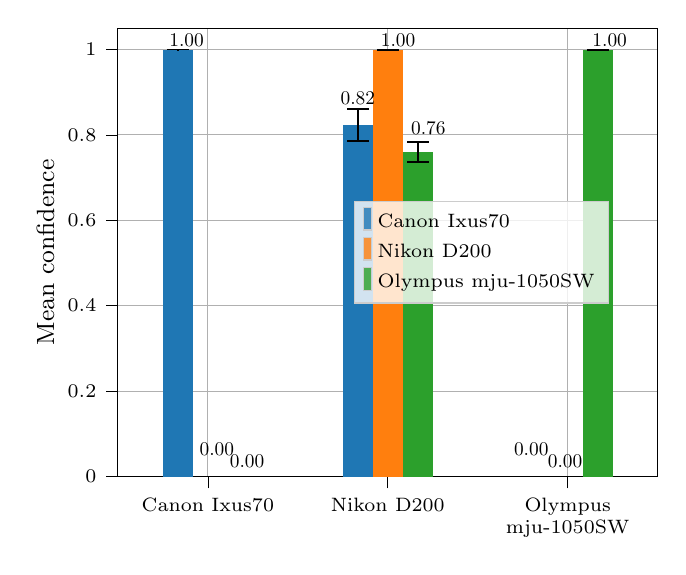
\begin{tikzpicture}

\definecolor{color0}{rgb}{0.12156862745098,0.466666666666667,0.705882352941177}
\definecolor{color1}{rgb}{1,0.498039215686275,0.0549019607843137}
\definecolor{color2}{rgb}{0.172549019607843,0.627450980392157,0.172549019607843}

\pgfplotsset{compat=1.11,
	/pgfplots/ybar legend/.style={
		/pgfplots/legend image code/.code={%
			\draw[##1,/tikz/.cd,yshift=-0.25em]
			(0cm,0cm) rectangle (3pt,0.8em);},
	},
	every tick label/.append style={font=\scriptsize}
}

\begin{axis}[
legend cell align={left},
legend style={fill opacity=0.8, draw opacity=1, text opacity=1, at={(0.91,0.5)}, anchor=east, draw=white!80!black},
tick align=outside,
tick pos=left,
grid=major,
x grid style={white!69.0196078431373!black},
xmin=-0.5, xmax=2.5,
xtick style={color=black},
xtick={0,1,2},
xticklabel style = {text width=2cm, align=center},
xticklabels={Canon Ixus70, Nikon D200, Olympus mju-1050SW},
y grid style={white!69.0196078431373!black},
ymin=0, ymax=1.04966682860504,
ytick style={color=black},
y label style={at={(axis description cs:-0.1,.5)},anchor=south},
ylabel={\small Mean confidence}
]
\draw[draw=none,fill=color0] (axis cs:-0.25,0) rectangle (axis cs:-0.0833333333333333,0.999627947807312);
\addlegendimage{ybar,ybar legend,draw=none,fill=color0};
\addlegendentry{\scriptsize Canon Ixus70}

\draw[draw=none,fill=color0] (axis cs:0.75,0) rectangle (axis cs:0.916666666666667,0.823229551315308);
\draw[draw=none,fill=color0] (axis cs:1.75,0) rectangle (axis cs:1.91666666666667,0);
\draw[draw=none,fill=color1] (axis cs:-0.0833333333333333,0) rectangle (axis cs:0.0833333333333333,0);
\addlegendimage{ybar,ybar legend,draw=none,fill=color1};
\addlegendentry{\scriptsize Nikon D200}

\draw[draw=none,fill=color1] (axis cs:0.916666666666667,0) rectangle (axis cs:1.08333333333333,0.998548150062561);
\draw[draw=none,fill=color1] (axis cs:1.91666666666667,0) rectangle (axis cs:2.08333333333333,0);
\draw[draw=none,fill=color2] (axis cs:0.0833333333333333,0) rectangle (axis cs:0.25,0);
\addlegendimage{ybar,ybar legend,draw=none,fill=color2};
\addlegendentry{\scriptsize Olympus mju-1050SW}

\draw[draw=none,fill=color2] (axis cs:1.08333333333333,0) rectangle (axis cs:1.25,0.759181141853333);
\draw[draw=none,fill=color2] (axis cs:2.08333333333333,0) rectangle (axis cs:2.25,0.998918771743774);
\path [draw=black, semithick]
(axis cs:-0.166666666666667,0.999573201705061)
--(axis cs:-0.166666666666667,0.999682693909563);

\path [draw=black, semithick]
(axis cs:0.833333333333333,0.785822704434395)
--(axis cs:0.833333333333333,0.86063639819622);

\path [draw=black, semithick]
(axis cs:1.83333333333333,0)
--(axis cs:1.83333333333333,0);

\path [draw=black, semithick]
(axis cs:0,0)
--(axis cs:0,0);

\path [draw=black, semithick]
(axis cs:1,0.998303965490777)
--(axis cs:1,0.998792334634345);

\path [draw=black, semithick]
(axis cs:2,0)
--(axis cs:2,0);

\path [draw=black, semithick]
(axis cs:0.166666666666667,0)
--(axis cs:0.166666666666667,0);

\path [draw=black, semithick]
(axis cs:1.16666666666667,0.735817492008209)
--(axis cs:1.16666666666667,0.782544791698456);

\path [draw=black, semithick]
(axis cs:2.16666666666667,0.998699586911243)
--(axis cs:2.16666666666667,0.999137956576305);

\addplot [semithick, black, mark=-, mark size=4, mark options={solid}, only marks]
table {%
-0.166666666666667 0.999573201705061
0.833333333333333 0.785822704434395
1.83333333333333 0
};

\addplot [semithick, black, mark=-, mark size=4, mark options={solid}, only marks]
table {%
-0.166666666666667 0.999682693909563
0.833333333333333 0.86063639819622
1.83333333333333 0
};

\addplot [semithick, black, mark=-, mark size=4, mark options={solid}, only marks]
table {%
0 0
1 0.998303965490777
2 0
};

\addplot [semithick, black, mark=-, mark size=4, mark options={solid}, only marks]
table {%
0 0
1 0.998792334634345
2 0
};

\addplot [semithick, black, mark=-, mark size=4, mark options={solid}, only marks]
table {%
0.166666666666667 0
1.16666666666667 0.735817492008209
2.16666666666667 0.998699586911243
};

\addplot [semithick, black, mark=-, mark size=4, mark options={solid}, only marks]
table {%
0.166666666666667 0
1.16666666666667 0.782544791698456
2.16666666666667 0.999137956576305
};

\draw (axis cs:-0.252,1.00762497138977) node[
scale=0.7,
anchor=base west,
text=black,
rotate=0.0
]{1.00};
\draw (axis cs:0.7,0.87) node[
scale=0.7,
anchor=base west,
text=black,
rotate=0.0
]{0.82};
\draw (axis cs:1.664,0.05) node[
scale=0.7,
anchor=base west,
text=black,
rotate=0.0
]{0.00};
\draw (axis cs:-0.084,0.05) node[
scale=0.7,
anchor=base west,
text=black,
rotate=0.0
]{0.00};
\draw (axis cs:0.924,1.00653653526306) node[
scale=0.7,
anchor=base west,
text=black,
rotate=0.0
]{1.00};
\draw (axis cs:1.852,0.02) node[
scale=0.7,
anchor=base west,
text=black,
rotate=0.0
]{0.00};
\draw (axis cs:0.084,0.02) node[
scale=0.7,
anchor=base west,
text=black,
rotate=0.0
]{0.00};
\draw (axis cs:1.092,0.8) node[
scale=0.7,
anchor=base west,
text=black,
rotate=0.0
]{0.76};
\draw (axis cs:2.1,1.00691012191772) node[
scale=0.7,
anchor=base west,
text=black,
rotate=0.0
]{1.00};

\end{axis}

\end{tikzpicture}
}
	}
	\caption{Mean prediction confidence to test data, x axis indicates the images from three testing models, y axis shows the value of mean prediction confidence. The color bars tell us which model the image is classified into.}
	\label{fig:test confidence}
\end{figure}

%%%%%%%%%%%%%%%%%%%%%%%%%%%%%%%%%%%%%%%%%%%%%%%%%%%%%%%%%%%%%%%%%%%%%%%%%%%%%%
\subsection{Unseen camera models}
\label{section:unseen}
%%%%%%%%%%%%%%%%%%%%%%%%%%%%%%%%%%%%%%%%%%%%%%%%%%%%%%%%%%%%%%%%%%%%%%%%%%%%%%

This experiment is to test the impact of images from unseen camera models on the robustness of our classifier. The goal of this experiment is to see how our CNN classifies the images from unseen camera models. Note that in this experiment our model classifies the input images from the five testing camera models as one of the three training camera models, as we trained our model on a closed set classification task using the mutual exclusive class labels $\mathcal{C} = \{\text{Canon Ixus70}, \text{Nikon D200}, \text{Olympus mju-1050SW}\}$. Since the ground truth is different from the label set $\mathcal{C}$, the classifier should make decision without high confidence if it is robust to images from unseen camera models. It could be interpreted that the classifier cannot be sure which model the image comes from.

%%%%%%%%%%%%%%%%%%%%%%%%%%%%%%%%%%%%%%%%%%%%%%%%%%%%%%%%%%%%%%%%%%%%%%%%%%%%%%
\subsection*{Data collection}
\label{section:unseen data collection & Training}
%%%%%%%%%%%%%%%%%%%%%%%%%%%%%%%%%%%%%%%%%%%%%%%%%%%%%%%%%%%%%%%%%%%%%%%%%%%%%%

As shown in Table \ref{tab:makes}, we choose five more models in the dresden image database, which are \textbf{Agfa DC-830i}, \textbf{Canon Ixus55}, \textbf{Canon PowershotA640}, \textbf{Nikon D70} and \textbf{Sony W170}. In order to see if the brand and image content affect the result of our classifier, these five models have different relations to the training models in terms of brand and image contents. These 1,549 images are also divided into $ 256 \times 256 $ patches in the same manner mentioned before. In total, our unseen database consists of 38,725 patches.

\begin{table}
	\center
	\begin{tabular}{ |p{2.8cm}|p{1.1cm}|p{1.2cm}|p{1.6cm}| }
		\hline
		Camera Models & Brand & Contents & Number of images\\
		\hline
		Agfa DC-830i & different & similar & 363 \\
		Canon Ixus55 & same & similar & 224 \\
		Canon Powershot64 & same & different & 188 \\
		Nikon D70 & same & similar & 369 \\
		Sony W170 & different & different & 405 \\
		\hline
		\multicolumn{3}{|c|}{Total number of images} & 1,549 \\
		\hline
	\end{tabular}
	\caption{\label{tab:makes} Five unseen camera models with different relations in terms of brand and image's content. The rightmost column shows the number of testing images from the corresponding camera model. Note that the images here are full sized images.}
\end{table}

%%%%%%%%%%%%%%%%%%%%%%%%%%%%%%%%%%%%%%%%%%%%%%%%%%%%%%%%%%%%%%%%%%%%%%%%%%%%%%
\subsection*{Result}
\label{section:unseen result}
%%%%%%%%%%%%%%%%%%%%%%%%%%%%%%%%%%%%%%%%%%%%%%%%%%%%%%%%%%%%%%%%%%%%%%%%%%%%%%

We randomly selected 6,400 patches from our unseen database, and evaluate the classifier's most likely class prediction, as well as its prediction confidence, which is shown in Figure \ref{fig:unseen result} and \ref{fig:unseen confidence}, respectively. 

\begin{figure}
	\centering
	\resizebox{!}{!}{
		{% This file was created by tikzplotlib v0.9.1.
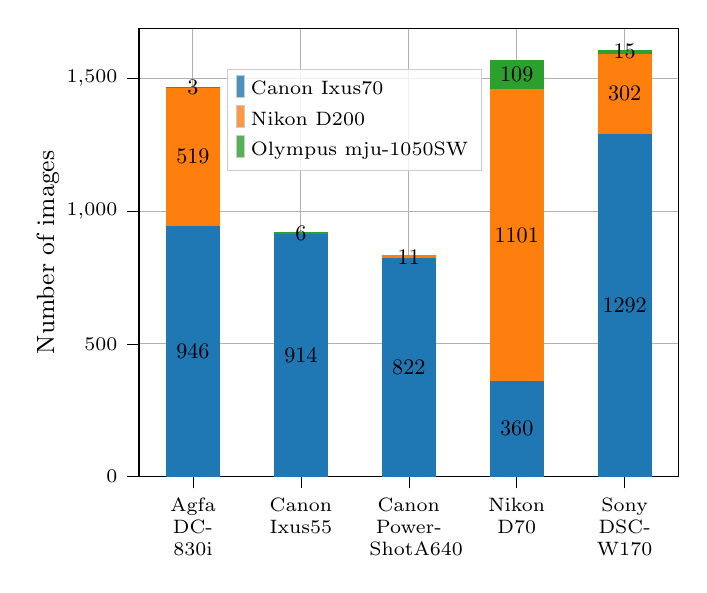
\begin{tikzpicture}

\definecolor{color0}{rgb}{0.12156862745098,0.466666666666667,0.705882352941177}
\definecolor{color1}{rgb}{1,0.498039215686275,0.0549019607843137}
\definecolor{color2}{rgb}{0.172549019607843,0.627450980392157,0.172549019607843}

\pgfplotsset{compat=1.11,
	/pgfplots/ybar legend/.style={
		/pgfplots/legend image code/.code={%
			\draw[##1,/tikz/.cd,yshift=-0.25em]
			(0cm,0cm) rectangle (3pt,0.8em);},
	}, every tick label/.append style={font=\scriptsize}
}

\begin{axis}[
legend cell align={left},
legend style={fill opacity=0.8, draw opacity=1, text opacity=1, at={(0.4,0.91)}, anchor=north, draw=white!80!black},
tick align=outside,
tick pos=left,
grid=major,
x grid style={white!69.0196078431373!black},
xmin=-0.5, xmax=4.5,
xtick style={color=black},
xtick={0,1,2,3,4},
xticklabel style={text width=1cm, align=center},
xticklabels={Agfa DC-830i, Canon Ixus55, Canon PowerShotA640, Nikon D70, Sony DSC-W170},
y grid style={white!69.0196078431373!black},
ymin=0, ymax=1689.45,
ytick style={color=black},
y label style={at={(axis description cs:-0.13,.5)},anchor=south},
ylabel={\small Number of images}
]
\draw[draw=none,fill=color0] (axis cs:-0.25,0) rectangle (axis cs:0.25,946);
\addlegendimage{ybar,ybar legend,draw=none,fill=color0};
\addlegendentry{\scriptsize Canon Ixus70}

\draw[draw=none,fill=color0] (axis cs:0.75,0) rectangle (axis cs:1.25,914);
\draw[draw=none,fill=color0] (axis cs:1.75,0) rectangle (axis cs:2.25,822);
\draw[draw=none,fill=color0] (axis cs:2.75,0) rectangle (axis cs:3.25,360);
\draw[draw=none,fill=color0] (axis cs:3.75,0) rectangle (axis cs:4.25,1292);
\draw[draw=none,fill=color1] (axis cs:-0.25,946) rectangle (axis cs:0.25,1465);
\addlegendimage{ybar,ybar legend,draw=none,fill=color1};
\addlegendentry{\scriptsize Nikon D200}

\draw[draw=none,fill=color1] (axis cs:0.75,0) rectangle (axis cs:1.25,0);
\draw[draw=none,fill=color1] (axis cs:1.75,822) rectangle (axis cs:2.25,833);
\draw[draw=none,fill=color1] (axis cs:2.75,360) rectangle (axis cs:3.25,1461);
\draw[draw=none,fill=color1] (axis cs:3.75,1292) rectangle (axis cs:4.25,1594);
\draw[draw=none,fill=color2] (axis cs:-0.25,1465) rectangle (axis cs:0.25,1468);
\addlegendimage{ybar,ybar legend,draw=none,fill=color2};
\addlegendentry{\scriptsize Olympus mju-1050SW}

\draw[draw=none,fill=color2] (axis cs:0.75,914) rectangle (axis cs:1.25,920);
\draw[draw=none,fill=color2] (axis cs:1.75,0) rectangle (axis cs:2.25,0);
\draw[draw=none,fill=color2] (axis cs:2.75,1461) rectangle (axis cs:3.25,1570);
\draw[draw=none,fill=color2] (axis cs:3.75,1594) rectangle (axis cs:4.25,1609);
\draw (axis cs:0,473) node[
  scale=0.8,
  text=black,
  rotate=0.0
]{946};
\draw (axis cs:1,457) node[
  scale=0.8,
  text=black,
  rotate=0.0
]{914};
\draw (axis cs:2,411) node[
  scale=0.8,
  text=black,
  rotate=0.0
]{822};
\draw (axis cs:3,180) node[
  scale=0.8,
  text=black,
  rotate=0.0
]{360};
\draw (axis cs:4,646) node[
  scale=0.8,
  text=black,
  rotate=0.0
]{1292};
\draw (axis cs:0,1205.5) node[
  scale=0.8,
  text=black,
  rotate=0.0
]{519};
\draw (axis cs:2,827.5) node[
  scale=0.8,
  text=black,
  rotate=0.0
]{11};
\draw (axis cs:3,910.5) node[
  scale=0.8,
  text=black,
  rotate=0.0
]{1101};
\draw (axis cs:4,1443) node[
  scale=0.8,
  text=black,
  rotate=0.0
]{302};
\draw (axis cs:0,1466.5) node[
  scale=0.8,
  text=black,
  rotate=0.0
]{3};
\draw (axis cs:1,917) node[
  scale=0.8,
  text=black,
  rotate=0.0
]{6};
\draw (axis cs:3,1515.5) node[
  scale=0.8,
  text=black,
  rotate=0.0
]{109};
\draw (axis cs:4,1601.5) node[
  scale=0.8,
  text=black,
  rotate=0.0
]{15};
\end{axis}

\end{tikzpicture}
}
	}
	\caption{Prediction to five unseen models. The numbers on the bars indicate the number of images that are classified to the corresponding classes.}
	\label{fig:unseen result}
\end{figure} 

We can notice that for the two Canon cameras, Canon Ixus55 and Canon PowerShotA640, our model classifies almost all the images from these two models as Canon Ixus 70, which has the same manufacturer as the two models. The mean prediction confidence of Canon Ixus55 and Canon PowerShotA640 are both equal or higher than $ 0.91 $, so it implies that the classifier is confident about the decisions it makes. However, there is difference between the prediction result of these two camera models. For the images from Canon Ixus55, the classifier tends to classify a small number of images as Olympus mju-1050SW, while for images from Canon PowerShotA640, as Nikon D200. In addition, the image contents of Canon Ixus55 are similar to the training set while Canon PowerShotA640 are different. Nevertheless, it seems this difference does not affect the result of these two camera models' images.

\begin{figure}
	\centering
	\resizebox{!}{!}{
		{% This file was created by tikzplotlib v0.9.1.
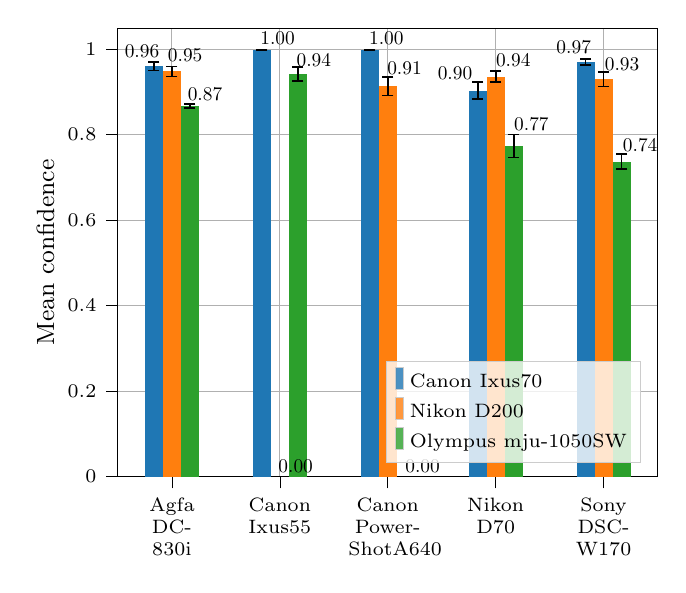
\begin{tikzpicture}

\definecolor{color0}{rgb}{0.12156862745098,0.466666666666667,0.705882352941177}
\definecolor{color1}{rgb}{1,0.498039215686275,0.0549019607843137}
\definecolor{color2}{rgb}{0.172549019607843,0.627450980392157,0.172549019607843}

\pgfplotsset{compat=1.11,
	/pgfplots/ybar legend/.style={
		/pgfplots/legend image code/.code={%
			\draw[##1,/tikz/.cd,yshift=-0.25em]
			(0cm,0cm) rectangle (3pt,0.8em);},
	}, every tick label/.append style={font=\scriptsize}
}

\begin{axis}[
legend cell align={left},
legend style={fill opacity=0.8, draw opacity=1, text opacity=1, at={(0.97,0.03)}, anchor=south east, draw=white!80!black},
tick align=outside,
tick pos=left,
grid=major,
x grid style={white!69.0196078431373!black},
xmin=-0.5, xmax=4.5,
xtick style={color=black},
xtick={0,1,2,3,4},
xticklabel style={text width=1cm, align=center},
xticklabels={Agfa DC-830i,Canon Ixus55,Canon PowerShotA640,Nikon D70,Sony DSC-W170},
y grid style={white!69.0196078431373!black},
ymin=0, ymax=1.04887666648719,
ytick style={color=black},
y label style={at={(axis description cs:-0.1,.5)},anchor=south},
ylabel={\small Mean confidence}
]
\draw[draw=none,fill=color0] (axis cs:-0.25,0) rectangle (axis cs:-0.0833333333333333,0.960057199001312);
\addlegendimage{ybar,ybar legend,draw=none,fill=color0};
\addlegendentry{\scriptsize Canon Ixus70}

\draw[draw=none,fill=color0] (axis cs:0.75,0) rectangle (axis cs:0.916666666666667,0.998571991920471);
\draw[draw=none,fill=color0] (axis cs:1.75,0) rectangle (axis cs:1.91666666666667,0.998243570327759);
\draw[draw=none,fill=color0] (axis cs:2.75,0) rectangle (axis cs:2.91666666666667,0.902838289737701);
\draw[draw=none,fill=color0] (axis cs:3.75,0) rectangle (axis cs:3.91666666666667,0.969556868076324);
\draw[draw=none,fill=color1] (axis cs:-0.0833333333333333,0) rectangle (axis cs:0.0833333333333333,0.947647273540497);
\addlegendimage{ybar,ybar legend,draw=none,fill=color1};
\addlegendentry{\scriptsize Nikon D200}

\draw[draw=none,fill=color1] (axis cs:0.916666666666667,0) rectangle (axis cs:1.08333333333333,0);
\draw[draw=none,fill=color1] (axis cs:1.91666666666667,0) rectangle (axis cs:2.08333333333333,0.912966668605804);
\draw[draw=none,fill=color1] (axis cs:2.91666666666667,0) rectangle (axis cs:3.08333333333333,0.935871481895447);
\draw[draw=none,fill=color1] (axis cs:3.91666666666667,0) rectangle (axis cs:4.08333333333333,0.928948819637299);
\draw[draw=none,fill=color2] (axis cs:0.0833333333333333,0) rectangle (axis cs:0.25,0.867151260375977);
\addlegendimage{ybar,ybar legend,draw=none,fill=color2};
\addlegendentry{\scriptsize Olympus mju-1050SW}

\draw[draw=none,fill=color2] (axis cs:1.08333333333333,0) rectangle (axis cs:1.25,0.941826820373535);
\draw[draw=none,fill=color2] (axis cs:2.08333333333333,0) rectangle (axis cs:2.25,0);
\draw[draw=none,fill=color2] (axis cs:3.08333333333333,0) rectangle (axis cs:3.25,0.773304998874664);
\draw[draw=none,fill=color2] (axis cs:4.08333333333333,0) rectangle (axis cs:4.25,0.736984550952911);
\path [draw=black, semithick]
(axis cs:-0.166666666666667,0.949836290441453)
--(axis cs:-0.166666666666667,0.970278107561171);

\path [draw=black, semithick]
(axis cs:0.833333333333333,0.998213825281709)
--(axis cs:0.833333333333333,0.998930158559233);

\path [draw=black, semithick]
(axis cs:1.83333333333333,0.997746782202739)
--(axis cs:1.83333333333333,0.998740358452778);

\path [draw=black, semithick]
(axis cs:2.83333333333333,0.883183458819985)
--(axis cs:2.83333333333333,0.922493120655417);

\path [draw=black, semithick]
(axis cs:3.83333333333333,0.962237296625972)
--(axis cs:3.83333333333333,0.976876439526677);

\path [draw=black, semithick]
(axis cs:0,0.935686012730002)
--(axis cs:0,0.959608534350991);

\path [draw=black, semithick]
(axis cs:1,0)
--(axis cs:1,0);

\path [draw=black, semithick]
(axis cs:2,0.891556613147259)
--(axis cs:2,0.93437672406435);

\path [draw=black, semithick]
(axis cs:3,0.92278899345547)
--(axis cs:3,0.948953970335424);

\path [draw=black, semithick]
(axis cs:4,0.912190033122897)
--(axis cs:4,0.9457076061517);

\path [draw=black, semithick]
(axis cs:0.166666666666667,0.862032268662006)
--(axis cs:0.166666666666667,0.872270252089947);

\path [draw=black, semithick]
(axis cs:1.16666666666667,0.925926184281707)
--(axis cs:1.16666666666667,0.957727456465364);

\path [draw=black, semithick]
(axis cs:2.16666666666667,0)
--(axis cs:2.16666666666667,0);

\path [draw=black, semithick]
(axis cs:3.16666666666667,0.746303979307413)
--(axis cs:3.16666666666667,0.800306018441916);

\path [draw=black, semithick]
(axis cs:4.16666666666667,0.71960430033505)
--(axis cs:4.16666666666667,0.754364801570773);

\addplot [semithick, black, mark=-, mark size=2, mark options={solid}, only marks]
table {%
-0.166666666666667 0.949836290441453
0.833333333333333 0.998213825281709
1.83333333333333 0.997746782202739
2.83333333333333 0.883183458819985
3.83333333333333 0.962237296625972
};

\addplot [semithick, black, mark=-, mark size=2, mark options={solid}, only marks]
table {%
-0.166666666666667 0.970278107561171
0.833333333333333 0.998930158559233
1.83333333333333 0.998740358452778
2.83333333333333 0.922493120655417
3.83333333333333 0.976876439526677
};

\addplot [semithick, black, mark=-, mark size=2, mark options={solid}, only marks]
table {%
0 0.935686012730002
1 0
2 0.891556613147259
3 0.92278899345547
4 0.912190033122897
};

\addplot [semithick, black, mark=-, mark size=2, mark options={solid}, only marks]
table {%
0 0.959608534350991
1 0
2 0.93437672406435
3 0.948953970335424
4 0.9457076061517
};

\addplot [semithick, black, mark=-, mark size=2, mark options={solid}, only marks]
table {%
0.166666666666667 0.862032268662006
1.16666666666667 0.925926184281707
2.16666666666667 0
3.16666666666667 0.746303979307413
4.16666666666667 0.71960430033505
};

\addplot [semithick, black, mark=-, mark size=2, mark options={solid}, only marks]
table {%
0.166666666666667 0.872270252089947
1.16666666666667 0.957727456465364
2.16666666666667 0
3.16666666666667 0.800306018441916
4.16666666666667 0.754364801570773
};

\draw (axis cs:-0.5,0.98) node[
  scale=0.7,
  anchor=base west,
  text=black,
  rotate=0.0
]{0.96};
\draw (axis cs:0.756,1.01) node[
  scale=0.7,
  anchor=base west,
  text=black,
  rotate=0.0
]{1.00};
\draw (axis cs:1.764,1.01) node[
  scale=0.7,
  anchor=base west,
  text=black,
  rotate=0.0
]{1.00};
\draw (axis cs:2.4,0.93) node[
  scale=0.7,
  anchor=base west,
  text=black,
  rotate=0.0
]{0.90};
\draw (axis cs:3.5,0.99) node[
  scale=0.7,
  anchor=base west,
  text=black,
  rotate=0.0
]{0.97};
\draw (axis cs:-0.1,0.97) node[
  scale=0.7,
  anchor=base west,
  text=black,
  rotate=0.0
]{0.95};
\draw (axis cs:0.924,0.01) node[
  scale=0.7,
  anchor=base west,
  text=black,
  rotate=0.0
]{0.00};
\draw (axis cs:1.932,0.94) node[
  scale=0.7,
  anchor=base west,
  text=black,
  rotate=0.0
]{0.91};
\draw (axis cs:2.94,0.96) node[
  scale=0.7,
  anchor=base west,
  text=black,
  rotate=0.0
]{0.94};
\draw (axis cs:3.948,0.95) node[
  scale=0.7,
  anchor=base west,
  text=black,
  rotate=0.0
]{0.93};
\draw (axis cs:0.084,0.88) node[
  scale=0.7,
  anchor=base west,
  text=black,
  rotate=0.0
]{0.87};
\draw (axis cs:1.092,0.96) node[
  scale=0.7,
  anchor=base west,
  text=black,
  rotate=0.0
]{0.94};
\draw (axis cs:2.1,0.01) node[
  scale=0.7,
  anchor=base west,
  text=black,
  rotate=0.0
]{0.00};
\draw (axis cs:3.108,0.81) node[
  scale=0.7,
  anchor=base west,
  text=black,
  rotate=0.0
]{0.77};
\draw (axis cs:4.116,0.76) node[
  scale=0.7,
  anchor=base west,
  text=black,
  rotate=0.0
]{0.74};
\end{axis}

\end{tikzpicture}
}
	}
	\caption{Mean prediction confidence to five unseen camera models.}
	\label{fig:unseen confidence}
\end{figure}

Similar result is also shown for images from Nikon D70. Our classifier tends to classify them as image from Nikon D200. It could be the reason that Nikon D70 and Nikon D200 both have the same manufacturer. As for rest 3,077 images from the other two camera models, Agfa DC-830i and Sony DSC-W170, out of these 2,238 are classified as Canon Ixus70, which makes about 72.7\%. Besides, when the classifier classifies the images from these three camera models as Canon Ixus70 and Nikon D200, it always has at least 0.90 mean prediction confidence. The mean prediction confidence to Olympus mju-1050SW is also considerable with a value higher than 0.74.

For all images of the unseen test models, the result doesn't show a relation to the image content. The explanation for this is the usage of constrained convolutional layer, which extract the high frequency characteristic of the camera instead of the scenes and objects of the images.

%%%%%%%%%%%%%%%%%%%%%%%%%%%%%%%%%%%%%%%%%%%%%%%%%%%%%%%%%%%%%%%%%%%%%%%%%%%%%%
\subsection*{Summary}
\label{section:unseen summary}
%%%%%%%%%%%%%%%%%%%%%%%%%%%%%%%%%%%%%%%%%%%%%%%%%%%%%%%%%%%%%%%%%%%%%%%%%%%%%%

In this set of experiment, we have shown that the CNN-based camera model classifier is affected by the manufacturer of the camera models and it is robust to the contents due to the constrained convolutional layer. However, the classifier makes wrong decision always with high confidence. To some extend, this classifier is not robust to unseen camera models, because it didn't show "hesitation" while making choices.

%%%%%%%%%%%%%%%%%%%%%%%%%%%%%%%%%%%%%%%%%%%%%%%%%%%%%%%%%%%%%%%%%%%%%%%%%%%%%%
\subsection{Post-processed images}
\label{section:post-pro	cessed}
%%%%%%%%%%%%%%%%%%%%%%%%%%%%%%%%%%%%%%%%%%%%%%%%%%%%%%%%%%%%%%%%%%%%%%%%%%%%%%

In experiment of \textbf{post-processed images}, we perform three different post-processing techniques on the images from the testing set respectively. The post-processing and their parameters are shown in Table~\ref{tab:post}. The parameters of these operations are referenced from the manipulation detection experiment by \citeauthor{bayar2017design} \cite{bayar2017design}.

\begin{table}
	\center
	\begin{tabular}{|p{3cm}|p{3cm}|}
		\hline
		Operations & Parameters \\
		\hline
		JPEG compression & $QF = 70$ \\
		Gaussian Noise & $\sigma = 2$ \\
		Gaussian Blur & $\sigma = 1.1$, $K_{size} = 5 \times 5$ \\
		\hline
	\end{tabular}
	\caption{\label{tab:post} Operations and parameters of the post-processing experiment. The parameters are referenced from the manipulation detection experiment by \citeauthor{bayar2017design} \cite{bayar2017design}.}
\end{table}

%%%%%%%%%%%%%%%%%%%%%%%%%%%%%%%%%%%%%%%%%%%%%%%%%%%%%%%%%%%%%%%%%%%%%%%%%%%%%%
\subsubsection{JPEG Compression}
\label{section:jpeg}
%%%%%%%%%%%%%%%%%%%%%%%%%%%%%%%%%%%%%%%%%%%%%%%%%%%%%%%%%%%%%%%%%%%%%%%%%%%%%%

We perform JPEG compression with a quality factor of 70 on all the patches from our test database. In the evaluation stage, we randomly choose 6,400 patches as input to our CNN.

%%%%%%%%%%%%%%%%%%%%%%%%%%%%%%%%%%%%%%%%%%%%%%%%%%%%%%%%%%%%%%%%%%%%%%%%%%%%%%
\paragraph{Result}
\label{section:jpeg result}
%%%%%%%%%%%%%%%%%%%%%%%%%%%%%%%%%%%%%%%%%%%%%%%%%%%%%%%%%%%%%%%%%%%%%%%%%%%%%%

The classification result of JPEG images is shown in the Figure~\ref{fig:jpeg result}. Compared to the accuracy of Table~\ref{tab:train}, although they are all from the same camera models and also have the same image contents, the overall classification accuracy has dropped significantly after JPEG compression as shown in Table~\ref{tab:jpeg}.

The accuracy of Olympus mju-1050SW has dropped more than 40\%. For Canon Ixus70, it's even more than 50\%. Surprisingly, the accuracy of Nikon D200 only decreased by about 6.5\%, from 99.69\% to 93.21\%, which is much better than the other two models.

In terms of the prediction confidence, the mean confidences of the corresponding correct class are still the highest compared to the other two classes. So the classifier is still more certain when making the correct decision. But comparing Figure~\ref{fig:jpeg confidence} with the Figure~\ref{fig:test confidence}, it shows that not only the difference between these mean confidences become greatly smaller except for Nikon D200, but also the confidence for the corresponding correct class is decreased.

\begin{table}
	\center
	\begin{tabular}{ |p{3.2cm}|p{1.4cm}|p{2.6cm}| }
		\hline
		Camera Models & Accuracy & Number of images\\
		\hline
		Canon Ixus70 & 58.10\% & 1,439 \\
		Nikon D200 & 93.21\% & 1,886 \\
		Olympus mju-1050SW & 68.16\% & 3,075 \\
		\hline
		Overall Accuracy & \multicolumn{2}{c|}{73.16\%} \\
		\hline
	\end{tabular}
	\caption{\label{tab:jpeg} Prediction accuracy to JPEG compressed images with quality factor of 70. The images here are $ 256 \times 256 $ patches divided from full sized images.}
\end{table}

\begin{figure}
	\centering
	\resizebox{!}{!}{
		{% This file was created by tikzplotlib v0.9.1.
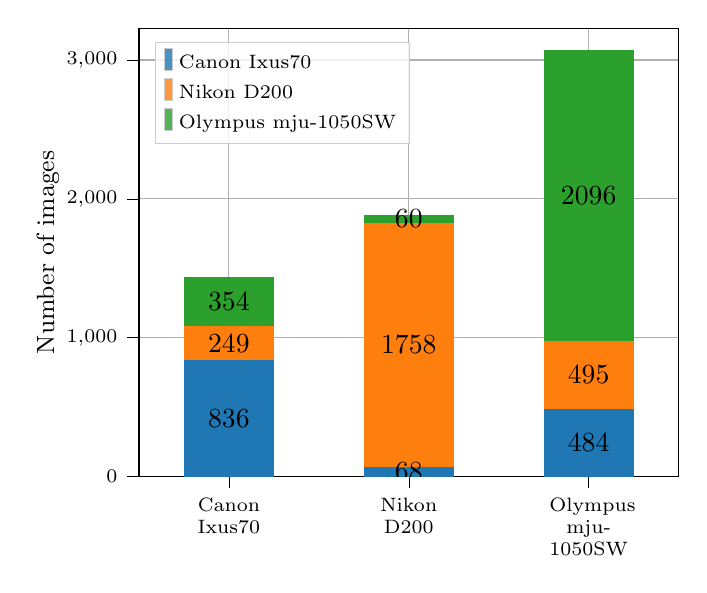
\begin{tikzpicture}

\definecolor{color0}{rgb}{0.12156862745098,0.466666666666667,0.705882352941177}
\definecolor{color1}{rgb}{1,0.498039215686275,0.0549019607843137}
\definecolor{color2}{rgb}{0.172549019607843,0.627450980392157,0.172549019607843}

\pgfplotsset{compat=1.11,
	/pgfplots/ybar legend/.style={
		/pgfplots/legend image code/.code={%
			\draw[##1,/tikz/.cd,yshift=-0.25em]
			(0cm,0cm) rectangle (3pt,0.8em);},
	}, every tick label/.append style={font=\scriptsize}
}

\begin{axis}[
legend cell align={left},
legend style={fill opacity=0.8, draw opacity=1, text opacity=1, at={(0.03,0.97)}, anchor=north west, draw=white!80!black},
tick align=outside,
tick pos=left,
grid=major,
x grid style={white!69.0196078431373!black},
xmin=-0.5, xmax=2.5,
xtick style={color=black},
xtick={0,1,2},
xticklabel style={text width=1cm, align=center},
xticklabels={Canon Ixus70,Nikon D200,Olympus mju-1050SW},
y grid style={white!69.0196078431373!black},
ymin=0, ymax=3228.75,
ytick style={color=black},
y label style={at={(axis description cs:-0.13,.5)},anchor=south},
ylabel={\small Number of images}
]
\draw[draw=none,fill=color0] (axis cs:-0.25,0) rectangle (axis cs:0.25,836);
\addlegendimage{ybar,ybar legend,draw=none,fill=color0};
\addlegendentry{\scriptsize Canon Ixus70}

\draw[draw=none,fill=color0] (axis cs:0.75,0) rectangle (axis cs:1.25,68);
\draw[draw=none,fill=color0] (axis cs:1.75,0) rectangle (axis cs:2.25,484);
\draw[draw=none,fill=color1] (axis cs:-0.25,836) rectangle (axis cs:0.25,1085);
\addlegendimage{ybar,ybar legend,draw=none,fill=color1};
\addlegendentry{\scriptsize Nikon D200}

\draw[draw=none,fill=color1] (axis cs:0.75,68) rectangle (axis cs:1.25,1826);
\draw[draw=none,fill=color1] (axis cs:1.75,484) rectangle (axis cs:2.25,979);
\draw[draw=none,fill=color2] (axis cs:-0.25,1085) rectangle (axis cs:0.25,1439);
\addlegendimage{ybar,ybar legend,draw=none,fill=color2};
\addlegendentry{\scriptsize Olympus mju-1050SW}

\draw[draw=none,fill=color2] (axis cs:0.75,1826) rectangle (axis cs:1.25,1886);
\draw[draw=none,fill=color2] (axis cs:1.75,979) rectangle (axis cs:2.25,3075);
\draw (axis cs:0,418) node[
  scale=1,
  text=black,
  rotate=0.0
]{836};
\draw (axis cs:1,34) node[
  scale=1,
  text=black,
  rotate=0.0
]{68};
\draw (axis cs:2,242) node[
  scale=1,
  text=black,
  rotate=0.0
]{484};
\draw (axis cs:0,960.5) node[
  scale=1,
  text=black,
  rotate=0.0
]{249};
\draw (axis cs:1,947) node[
  scale=1,
  text=black,
  rotate=0.0
]{1758};
\draw (axis cs:2,731.5) node[
  scale=1,
  text=black,
  rotate=0.0
]{495};
\draw (axis cs:0,1262) node[
  scale=1,
  text=black,
  rotate=0.0
]{354};
\draw (axis cs:1,1856) node[
  scale=1,
  text=black,
  rotate=0.0
]{60};
\draw (axis cs:2,2027) node[
  scale=1,
  text=black,
  rotate=0.0
]{2096};
\end{axis}

\end{tikzpicture}
}
	}
	\caption{Prediction of JPEG compressed images with quality factor of 70.}
	\label{fig:jpeg result}
\end{figure}

\begin{figure}
	\centering
	\resizebox{!}{!}{
		{% This file was created by tikzplotlib v0.9.1.
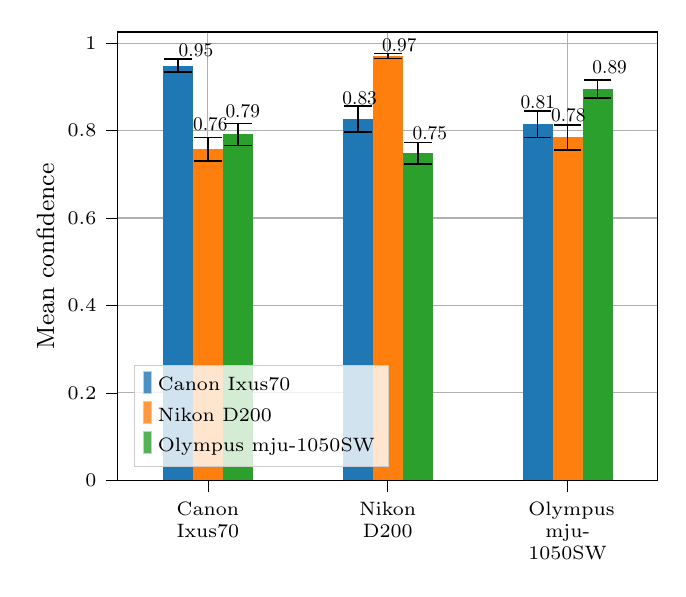
\begin{tikzpicture}

\definecolor{color0}{rgb}{0.12156862745098,0.466666666666667,0.705882352941177}
\definecolor{color1}{rgb}{1,0.498039215686275,0.0549019607843137}
\definecolor{color2}{rgb}{0.172549019607843,0.627450980392157,0.172549019607843}

\pgfplotsset{compat=1.11,
	/pgfplots/ybar legend/.style={
		/pgfplots/legend image code/.code={%
			\draw[##1,/tikz/.cd,yshift=-0.25em]
			(0cm,0cm) rectangle (3pt,0.8em);},
	}, every tick label/.append style={font=\scriptsize}
}

\begin{axis}[
legend cell align={left},
legend style={fill opacity=0.8, draw opacity=1, text opacity=1, at={(0.03,0.03)}, anchor=south west, draw=white!80!black},
tick align=outside,
tick pos=left,
grid=major,
x grid style={white!69.0196078431373!black},
xmin=-0.5, xmax=2.5,
xtick style={color=black},
xtick={0,1,2},
xticklabel style={text width=1cm, align=center},
xticklabels={Canon Ixus70,Nikon D200,Olympus mju-1050SW},
y grid style={white!69.0196078431373!black},
ymin=0, ymax=1.02536189903039,
ytick style={color=black},
y label style={at={(axis description cs:-0.1,.5)},anchor=south},
ylabel={\small Mean confidence}
]
\draw[draw=none,fill=color0] (axis cs:-0.25,0) rectangle (axis cs:-0.0833333333333333,0.948431253433228);
\addlegendimage{ybar,ybar legend,draw=none,fill=color0};
\addlegendentry{\scriptsize Canon Ixus70}

\draw[draw=none,fill=color0] (axis cs:0.75,0) rectangle (axis cs:0.916666666666667,0.826270997524261);
\draw[draw=none,fill=color0] (axis cs:1.75,0) rectangle (axis cs:1.91666666666667,0.814468204975128);
\draw[draw=none,fill=color1] (axis cs:-0.0833333333333333,0) rectangle (axis cs:0.0833333333333333,0.75765061378479);
\addlegendimage{ybar,ybar legend,draw=none,fill=color1};
\addlegendentry{\scriptsize Nikon D200}

\draw[draw=none,fill=color1] (axis cs:0.916666666666667,0) rectangle (axis cs:1.08333333333333,0.97075742483139);
\draw[draw=none,fill=color1] (axis cs:1.91666666666667,0) rectangle (axis cs:2.08333333333333,0.784488320350647);
\draw[draw=none,fill=color2] (axis cs:0.0833333333333333,0) rectangle (axis cs:0.25,0.791217505931854);
\addlegendimage{ybar,ybar legend,draw=none,fill=color2};
\addlegendentry{\scriptsize Olympus mju-1050SW}

\draw[draw=none,fill=color2] (axis cs:1.08333333333333,0) rectangle (axis cs:1.25,0.748564302921295);
\draw[draw=none,fill=color2] (axis cs:2.08333333333333,0) rectangle (axis cs:2.25,0.894988059997559);
\path [draw=black, semithick]
(axis cs:-0.166666666666667,0.933851783163846)
--(axis cs:-0.166666666666667,0.96301072370261);

\path [draw=black, semithick]
(axis cs:0.833333333333333,0.796050023287535)
--(axis cs:0.833333333333333,0.856491971760988);

\path [draw=black, semithick]
(axis cs:1.83333333333333,0.784555271267891)
--(axis cs:1.83333333333333,0.844381138682365);

\path [draw=black, semithick]
(axis cs:0,0.730917163193226)
--(axis cs:0,0.784384064376354);

\path [draw=black, semithick]
(axis cs:1,0.964979707729071)
--(axis cs:1,0.976535141933709);

\path [draw=black, semithick]
(axis cs:2,0.75550208799541)
--(axis cs:2,0.813474552705884);

\path [draw=black, semithick]
(axis cs:0.166666666666667,0.766115613281727)
--(axis cs:0.166666666666667,0.816319398581982);

\path [draw=black, semithick]
(axis cs:1.16666666666667,0.724309941753745)
--(axis cs:1.16666666666667,0.772818664088845);

\path [draw=black, semithick]
(axis cs:2.16666666666667,0.874373665079474)
--(axis cs:2.16666666666667,0.915602454915643);

\addplot [semithick, black, mark=-, mark size=5, mark options={solid}, only marks]
table {%
-0.166666666666667 0.933851783163846
0.833333333333333 0.796050023287535
1.83333333333333 0.784555271267891
};

\addplot [semithick, black, mark=-, mark size=5, mark options={solid}, only marks]
table {%
-0.166666666666667 0.96301072370261
0.833333333333333 0.856491971760988
1.83333333333333 0.844381138682365
};

\addplot [semithick, black, mark=-, mark size=5, mark options={solid}, only marks]
table {%
0 0.730917163193226
1 0.964979707729071
2 0.75550208799541
};

\addplot [semithick, black, mark=-, mark size=5, mark options={solid}, only marks]
table {%
0 0.784384064376354
1 0.976535141933709
2 0.813474552705884
};

\addplot [semithick, black, mark=-, mark size=5, mark options={solid}, only marks]
table {%
0.166666666666667 0.766115613281727
1.16666666666667 0.724309941753745
2.16666666666667 0.874373665079474
};

\addplot [semithick, black, mark=-, mark size=5, mark options={solid}, only marks]
table {%
0.166666666666667 0.816319398581982
1.16666666666667 0.772818664088845
2.16666666666667 0.915602454915643
};

\draw (axis cs:-0.20,0.97) node[
  scale=0.7,
  anchor=base west,
  text=black,
  rotate=0.0
]{0.95};
\draw (axis cs:0.71,0.86) node[
  scale=0.7,
  anchor=base west,
  text=black,
  rotate=0.0
]{0.83};
\draw (axis cs:1.7,0.85) node[
  scale=0.7,
  anchor=base west,
  text=black,
  rotate=0.0
]{0.81};
\draw (axis cs:-0.12,0.8) node[
  scale=0.7,
  anchor=base west,
  text=black,
  rotate=0.0
]{0.76};
\draw (axis cs:0.93,0.98) node[
  scale=0.7,
  anchor=base west,
  text=black,
  rotate=0.0
]{0.97};
\draw (axis cs:1.87,0.82) node[
  scale=0.7,
  anchor=base west,
  text=black,
  rotate=0.0
]{0.78};
\draw (axis cs:0.06,0.83) node[
  scale=0.7,
  anchor=base west,
  text=black,
  rotate=0.0
]{0.79};
\draw (axis cs:1.1,0.78) node[
  scale=0.7,
  anchor=base west,
  text=black,
  rotate=0.0
]{0.75};
\draw (axis cs:2.1,0.93) node[
  scale=0.7,
  anchor=base west,
  text=black,
  rotate=0.0
]{0.89};
\end{axis}

\end{tikzpicture}
}
	}
	\caption{Mean prediction confidence of JPEG compressed images with quality factor of 70.}
	\label{fig:jpeg confidence}
\end{figure}

%%%%%%%%%%%%%%%%%%%%%%%%%%%%%%%%%%%%%%%%%%%%%%%%%%%%%%%%%%%%%%%%%%%%%%%%%%%%%%
\paragraph{Summary}
\label{section:jpeg summary}
%%%%%%%%%%%%%%%%%%%%%%%%%%%%%%%%%%%%%%%%%%%%%%%%%%%%%%%%%%%%%%%%%%%%%%%%%%%%%%

The result of this experiment shows that, the classifier is robust to the JPEG compressed images from Nikon D200, but it fails when classifying the JPEG compressed images from the other two models. Considering the mean confidence when classifying Nikon D200's images in this experiment doesn't show great difference from Figure~\ref{fig:test confidence}, one possible explanation for the robustness of Nikon D200 is that compared to the high frequency characteristic left by the camera,  the artifacts caused by the jpeg compression are in different frequency range, such that the classifier consider these artifacts as unimportant when classifying images from Nikon D200. Nevertheless, when the classifier misclassifies images, it is always less sure about its decision compared to when it correctly classifies.

%%%%%%%%%%%%%%%%%%%%%%%%%%%%%%%%%%%%%%%%%%%%%%%%%%%%%%%%%%%%%%%%%%%%%%%%%%%%%%
\subsubsection{Additive Gaussian Noise}
\label{section:noise}
%%%%%%%%%%%%%%%%%%%%%%%%%%%%%%%%%%%%%%%%%%%%%%%%%%%%%%%%%%%%%%%%%%%%%%%%%%%%%%

A Gaussian noise with with zero mean and standard deviation of $ \sigma = 2 $ is added to the patch in the test database in this experiment. To evaluate the robustness of our classifier to additive Gaussian noise, we randomly select 6,400 patches from the test set and distort each patch with zero-mean additive Gaussian noise.

%%%%%%%%%%%%%%%%%%%%%%%%%%%%%%%%%%%%%%%%%%%%%%%%%%%%%%%%%%%%%%%%%%%%%%%%%%%%%%
\paragraph{Result}
\label{section:noise result}
%%%%%%%%%%%%%%%%%%%%%%%%%%%%%%%%%%%%%%%%%%%%%%%%%%%%%%%%%%%%%%%%%%%%%%%%%%%%%%

Figure~\ref{fig:noise result} and Table~\ref{tab:noise} show the classification result for these noisy images. In contrary to the JPEG compression experiment, the accuracy of Canon Ixus70 is nearly the same as in the baseline experiment, while the accuracies of Nikon D200 and Olympus mju-1050SW have downgraded severely, especially Olympus mju-1050SW, it decreases from 100\% to 23.53\%.

As shown in Figure~\ref{fig:noise confidence}, the prediction confidence for Canon Ixus70 doesn't change much as well. The mean confidence for classifying noisy Canon Ixus70 images as Canon Ixus70 images is still 1, and the 0.77 mean confidence for Nikon D200 is just caused by a very small number of misclassifications. When classifying images from the other two models, Nikon D200 and Olympus mju-1050SW, as Canon Ixus70 images, they both show more than 0.9 confidence to this wrong decision. In the case of Olympus mju-1050SW, the confidence is even higher compared to a correct decision. 

\begin{table}
	\center
	\begin{tabular}{ |p{3.2cm}|p{1.4cm}|p{2.6cm}| }
		\hline
		Camera Models & Accuracy & Number of images \\
		\hline
		Canon Ixus70 & 99.49\% & 1,371 \\
		Nikon D200 & 55.94\% & 1,977 \\
		Olympus mju-1050SW & 23.53\% & 3,052 \\
		\hline
		Overall Accuracy & \multicolumn{2}{c|}{59,65\%} \\
		\hline
	\end{tabular}
	\caption{\label{tab:noise} Prediction accuracy to images added Gaussian noise with zero-mean and standard deviation $ \sigma = 2 $. The images here are $ 256 \times 256 $ patches divided from full sized images.}
\end{table}

\begin{figure}
\centering
\resizebox{!}{!}{
	{% This file was created by tikzplotlib v0.9.1.
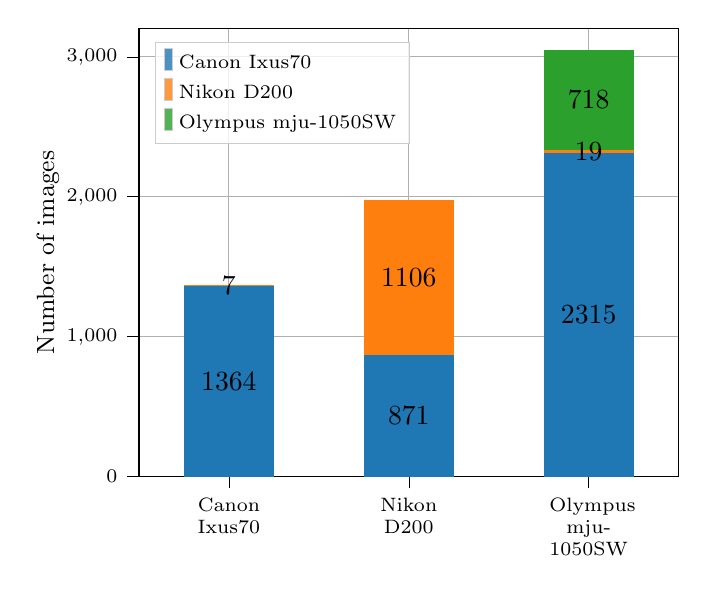
\begin{tikzpicture}

\definecolor{color0}{rgb}{0.12156862745098,0.466666666666667,0.705882352941177}
\definecolor{color1}{rgb}{1,0.498039215686275,0.0549019607843137}
\definecolor{color2}{rgb}{0.172549019607843,0.627450980392157,0.172549019607843}

\pgfplotsset{compat=1.11,
	/pgfplots/ybar legend/.style={
		/pgfplots/legend image code/.code={%
			\draw[##1,/tikz/.cd,yshift=-0.25em]
			(0cm,0cm) rectangle (3pt,0.8em);},
	}, every tick label/.append style={font=\scriptsize}
}

\begin{axis}[
legend cell align={left},
legend style={fill opacity=0.8, draw opacity=1, text opacity=1, at={(0.03,0.97)}, anchor=north west, draw=white!80!black},
tick align=outside,
tick pos=left,
grid=major,
x grid style={white!69.0196078431373!black},
xmin=-0.5, xmax=2.5,
xtick style={color=black},
xtick={0,1,2},
xticklabel style={text width=1cm, align=center},
xticklabels={Canon Ixus70,Nikon D200,Olympus mju-1050SW},
y grid style={white!69.0196078431373!black},
ymin=0, ymax=3204.6,
ytick style={color=black},
y label style={at={(axis description cs:-0.13,.5)},anchor=south},
ylabel={\small Number of images}
]
\draw[draw=none,fill=color0] (axis cs:-0.25,0) rectangle (axis cs:0.25,1364);
\addlegendimage{ybar,ybar legend,draw=none,fill=color0};
\addlegendentry{\scriptsize Canon Ixus70}

\draw[draw=none,fill=color0] (axis cs:0.75,0) rectangle (axis cs:1.25,871);
\draw[draw=none,fill=color0] (axis cs:1.75,0) rectangle (axis cs:2.25,2315);
\draw[draw=none,fill=color1] (axis cs:-0.25,1364) rectangle (axis cs:0.25,1371);
\addlegendimage{ybar,ybar legend,draw=none,fill=color1};
\addlegendentry{\scriptsize Nikon D200}

\draw[draw=none,fill=color1] (axis cs:0.75,871) rectangle (axis cs:1.25,1977);
\draw[draw=none,fill=color1] (axis cs:1.75,2315) rectangle (axis cs:2.25,2334);
\draw[draw=none,fill=color2] (axis cs:-0.25,0) rectangle (axis cs:0.25,0);
\addlegendimage{ybar,ybar legend,draw=none,fill=color2};
\addlegendentry{\scriptsize Olympus mju-1050SW}

\draw[draw=none,fill=color2] (axis cs:0.75,0) rectangle (axis cs:1.25,0);
\draw[draw=none,fill=color2] (axis cs:1.75,2334) rectangle (axis cs:2.25,3052);
\draw (axis cs:0,682) node[
  scale=1,
  text=black,
  rotate=0.0
]{1364};
\draw (axis cs:1,435.5) node[
  scale=1,
  text=black,
  rotate=0.0
]{871};
\draw (axis cs:2,1157.5) node[
  scale=1,
  text=black,
  rotate=0.0
]{2315};
\draw (axis cs:0,1367.5) node[
  scale=1,
  text=black,
  rotate=0.0
]{7};
\draw (axis cs:1,1424) node[
  scale=1,
  text=black,
  rotate=0.0
]{1106};
\draw (axis cs:2,2324.5) node[
  scale=1,
  text=black,
  rotate=0.0
]{19};
\draw (axis cs:2,2693) node[
  scale=1,
  text=black,
  rotate=0.0
]{718};
\end{axis}

\end{tikzpicture}
}
}
\caption{Prediction of images added Gaussian noise with zero-mean and standard deviation $ \sigma = 2 $.}
\label{fig:noise result}
\end{figure}


\begin{figure}
	\centering
	\resizebox{!}{!}{
		{% This file was created by tikzplotlib v0.9.1.
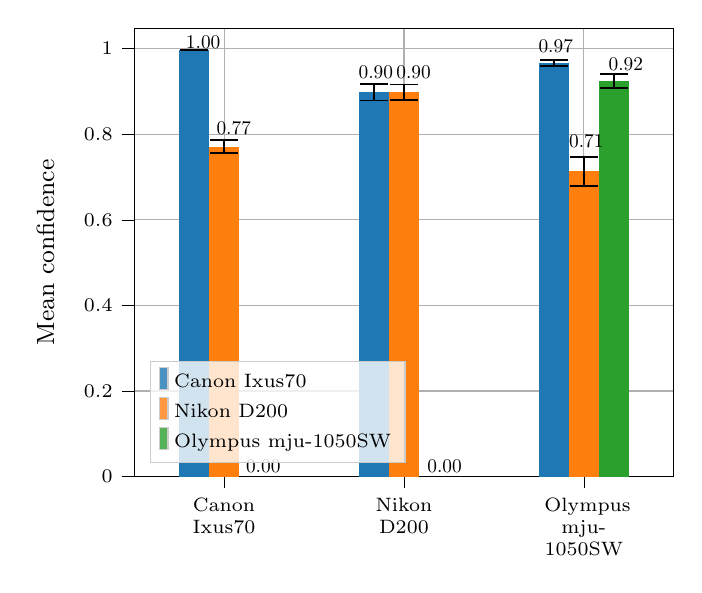
\begin{tikzpicture}

\definecolor{color0}{rgb}{0.12156862745098,0.466666666666667,0.705882352941177}
\definecolor{color1}{rgb}{1,0.498039215686275,0.0549019607843137}
\definecolor{color2}{rgb}{0.172549019607843,0.627450980392157,0.172549019607843}

\pgfplotsset{compat=1.11,
	/pgfplots/ybar legend/.style={
		/pgfplots/legend image code/.code={%
			\draw[##1,/tikz/.cd,yshift=-0.25em]
			(0cm,0cm) rectangle (3pt,0.8em);},
	}, every tick label/.append style={font=\scriptsize}
}

\begin{axis}[
legend cell align={left},
legend style={fill opacity=0.8, draw opacity=1, text opacity=1, at={(0.03,0.03)}, anchor=south west, draw=white!80!black},
tick align=outside,
tick pos=left,
grid=major,
x grid style={white!69.0196078431373!black},
xmin=-0.5, xmax=2.5,
xtick style={color=black},
xtick={0,1,2},
xticklabel style={text width=1cm, align=center},
xticklabels={Canon Ixus70,Nikon D200,Olympus mju-1050SW},
y grid style={white!69.0196078431373!black},
ymin=0, ymax=1.04788843104907,
ytick style={color=black},
y label style={at={(axis description cs:-0.13,.5)},anchor=south},
ylabel={\small Mean confidence}
]
\draw[draw=none,fill=color0] (axis cs:-0.25,0) rectangle (axis cs:-0.0833333333333333,0.997325718402863);
\addlegendimage{ybar,ybar legend,draw=none,fill=color0};
\addlegendentry{\scriptsize Canon Ixus70}

\draw[draw=none,fill=color0] (axis cs:0.75,0) rectangle (axis cs:0.916666666666667,0.898575067520142);
\draw[draw=none,fill=color0] (axis cs:1.75,0) rectangle (axis cs:1.91666666666667,0.966319143772125);
\draw[draw=none,fill=color1] (axis cs:-0.0833333333333333,0) rectangle (axis cs:0.0833333333333333,0.771355748176575);
\addlegendimage{ybar,ybar legend,draw=none,fill=color1};
\addlegendentry{\scriptsize Nikon D200}

\draw[draw=none,fill=color1] (axis cs:0.916666666666667,0) rectangle (axis cs:1.08333333333333,0.898063898086548);
\draw[draw=none,fill=color1] (axis cs:1.91666666666667,0) rectangle (axis cs:2.08333333333333,0.713302493095398);
\draw[draw=none,fill=color2] (axis cs:0.0833333333333333,0) rectangle (axis cs:0.25,0);
\addlegendimage{ybar,ybar legend,draw=none,fill=color2};
\addlegendentry{\scriptsize Olympus mju-1050SW}

\draw[draw=none,fill=color2] (axis cs:1.08333333333333,0) rectangle (axis cs:1.25,0);
\draw[draw=none,fill=color2] (axis cs:2.08333333333333,0) rectangle (axis cs:2.25,0.924066305160522);
\path [draw=black, semithick]
(axis cs:-0.166666666666667,0.996662454854231)
--(axis cs:-0.166666666666667,0.997988981951494);

\path [draw=black, semithick]
(axis cs:0.833333333333333,0.878918206319213)
--(axis cs:0.833333333333333,0.91823192872107);

\path [draw=black, semithick]
(axis cs:1.83333333333333,0.959143828600645)
--(axis cs:1.83333333333333,0.973494458943605);

\path [draw=black, semithick]
(axis cs:0,0.756258964538574)
--(axis cs:0,0.786452531814575);

\path [draw=black, semithick]
(axis cs:1,0.880109092220664)
--(axis cs:1,0.916018703952432);

\path [draw=black, semithick]
(axis cs:2,0.679081480950117)
--(axis cs:2,0.747523505240679);

\path [draw=black, semithick]
(axis cs:0.166666666666667,0)
--(axis cs:0.166666666666667,0);

\path [draw=black, semithick]
(axis cs:1.16666666666667,0)
--(axis cs:1.16666666666667,0);

\path [draw=black, semithick]
(axis cs:2.16666666666667,0.907951004803181)
--(axis cs:2.16666666666667,0.940181605517864);

\addplot [semithick, black, mark=-, mark size=5, mark options={solid}, only marks]
table {%
-0.166666666666667 0.996662454854231
0.833333333333333 0.878918206319213
1.83333333333333 0.959143828600645
};
 
\addplot [semithick, black, mark=-, mark size=5, mark options={solid}, only marks]
table {%
-0.166666666666667 0.997988981951494
0.833333333333333 0.91823192872107
1.83333333333333 0.973494458943605
};

\addplot [semithick, black, mark=-, mark size=5, mark options={solid}, only marks]
table {%
0 0.756258964538574
1 0.880109092220664
2 0.679081480950117
};
 
\addplot [semithick, black, mark=-, mark size=5, mark options={solid}, only marks]
table {%
0 0.786452531814575
1 0.916018703952432
2 0.747523505240679
};
 
\addplot [semithick, black, mark=-, mark size=5, mark options={solid}, only marks]
table {%
0.166666666666667 0
1.16666666666667 0
2.16666666666667 0.907951004803181
};
 
\addplot [semithick, black, mark=-, mark size=5, mark options={solid}, only marks]
table {%
0.166666666666667 0
1.16666666666667 0
2.16666666666667 0.940181605517864
};
 
\draw (axis cs:-0.25,1) node[
  scale=0.7,
  anchor=base west,
  text=black,
  rotate=0.0
]{1.00};
\draw (axis cs:0.71,0.93) node[
  scale=0.7,
  anchor=base west,
  text=black,
  rotate=0.0
]{0.90};
\draw (axis cs:1.71,0.99) node[
  scale=0.7,
  anchor=base west,
  text=black,
  rotate=0.0
]{0.97};
\draw (axis cs:-0.08,0.8) node[
  scale=0.7,
  anchor=base west,
  text=black,
  rotate=0.0
]{0.77};
\draw (axis cs:0.92,0.93) node[
  scale=0.7,
  anchor=base west,
  text=black,
  rotate=0.0
]{0.90};
\draw (axis cs:1.88,0.77) node[
  scale=0.7,
  anchor=base west,
  text=black,
  rotate=0.0
]{0.71};
\draw (axis cs:0.084,0.01) node[
  scale=0.7,
  anchor=base west,
  text=black,
  rotate=0.0
]{0.00};
\draw (axis cs:1.092,0.01) node[
  scale=0.7,
  anchor=base west,
  text=black,
  rotate=0.0
]{0.00};
\draw (axis cs:2.1,0.95) node[
  scale=0.7,
  anchor=base west,
  text=black,
  rotate=0.0
]{0.92};
\end{axis}

\end{tikzpicture}
}
	}
	\caption{Mean prediction confidence of images added Gaussian noise with zero-mean and standard deviation $ \sigma = 2 $.}
	\label{fig:noise confidence}
\end{figure}

%%%%%%%%%%%%%%%%%%%%%%%%%%%%%%%%%%%%%%%%%%%%%%%%%%%%%%%%%%%%%%%%%%%%%%%%%%%%%%
\paragraph{Summary}
\label{section:noise summary}
%%%%%%%%%%%%%%%%%%%%%%%%%%%%%%%%%%%%%%%%%%%%%%%%%%%%%%%%%%%%%%%%%%%%%%%%%%%%%%

In this experiment, it shows that the CNN-based camera model classifier is robust to additive Gaussian noise only for Canon Ixus70. For noisy images from the other two models, it tends to classify the noisy images as they are from Canon Ixus70 with high confidence. It leads to low accuracy for images from these models, especially for images from Olympus mju-1050SW. The explanation for this phenomenon could be that there is similarity between the high frequency characteristics of image from Canon Ixus70 and the Gaussian noise, such that it leads to the classifier tends to classify noisy image as Canon Ixus70's image.

%%%%%%%%%%%%%%%%%%%%%%%%%%%%%%%%%%%%%%%%%%%%%%%%%%%%%%%%%%%%%%%%%%%%%%%%%%%%%%
\subsubsection{Gaussian Blur}
\label{section:blur}
%%%%%%%%%%%%%%%%%%%%%%%%%%%%%%%%%%%%%%%%%%%%%%%%%%%%%%%%%%%%%%%%%%%%%%%%%%%%%%

A Gaussian blur operation with kernel's size of $ 5 \times 5 $ and standard deviation $ \sigma = 1.1 $ is performed on the image patches in the test database. We randomly select 6,400 patches and distort them with this Gaussian filter before using it as input to the classifier.

%%%%%%%%%%%%%%%%%%%%%%%%%%%%%%%%%%%%%%%%%%%%%%%%%%%%%%%%%%%%%%%%%%%%%%%%%%%%%%
\paragraph{Result}
\label{section:blur result}
%%%%%%%%%%%%%%%%%%%%%%%%%%%%%%%%%%%%%%%%%%%%%%%%%%%%%%%%%%%%%%%%%%%%%%%%%%%%%%

The result of this experiment is shown in Figure~\ref{fig:blur result} and Figure~\ref{fig:blur confidence}. Almost all images from these three models are classified as Nikon D200. The mean confidence for all images classified as Nikon D200 is 1, while for the other two models is low, which is either around 0.6 or 0.

\begin{figure}
	\centering
	\resizebox{!}{!}{
		{% This file was created by tikzplotlib v0.9.1.
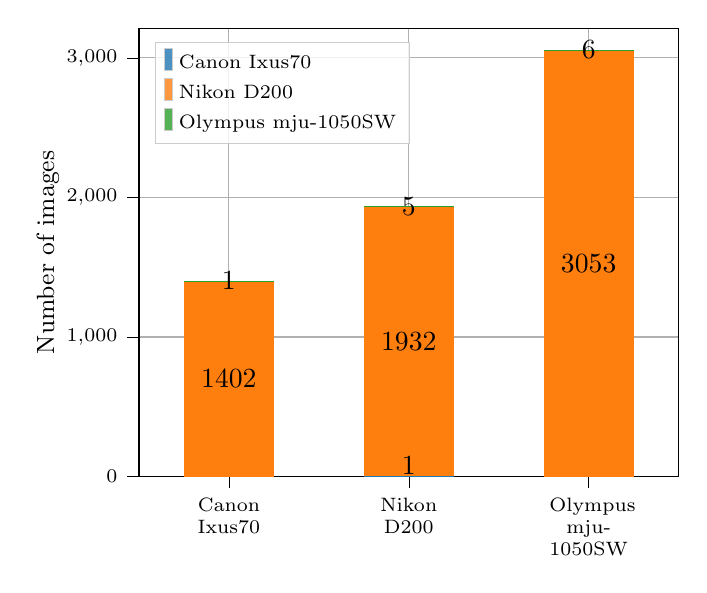
\begin{tikzpicture}

\definecolor{color0}{rgb}{0.12156862745098,0.466666666666667,0.705882352941177}
\definecolor{color1}{rgb}{1,0.498039215686275,0.0549019607843137}
\definecolor{color2}{rgb}{0.172549019607843,0.627450980392157,0.172549019607843}

\pgfplotsset{compat=1.11,
	/pgfplots/ybar legend/.style={
		/pgfplots/legend image code/.code={%
			\draw[##1,/tikz/.cd,yshift=-0.25em]
			(0cm,0cm) rectangle (3pt,0.8em);},
	}, every tick label/.append style={font=\scriptsize}
}

\begin{axis}[
legend cell align={left},
legend style={fill opacity=0.8, draw opacity=1, text opacity=1, at={(0.03,0.97)}, anchor=north west, draw=white!80!black},
tick align=outside,
tick pos=left,
grid=major,
x grid style={white!69.0196078431373!black},
xmin=-0.5, xmax=2.5,
xtick style={color=black},
xtick={0,1,2},
xticklabel style={text width=1cm, align=center},
xticklabels={Canon Ixus70,Nikon D200,Olympus mju-1050SW},
y grid style={white!69.0196078431373!black},
ymin=0, ymax=3211.95,
ytick style={color=black},
y label style={at={(axis description cs:-0.13,.5)},anchor=south},
ylabel={\small Number of images}
]
\draw[draw=none,fill=color0] (axis cs:-0.25,0) rectangle (axis cs:0.25,0);
\addlegendimage{ybar,ybar legend,draw=none,fill=color0};
\addlegendentry{\scriptsize Canon Ixus70}

\draw[draw=none,fill=color0] (axis cs:0.75,0) rectangle (axis cs:1.25,1);
\draw[draw=none,fill=color0] (axis cs:1.75,0) rectangle (axis cs:2.25,0);
\draw[draw=none,fill=color1] (axis cs:-0.25,0) rectangle (axis cs:0.25,1402);
\addlegendimage{ybar,ybar legend,draw=none,fill=color1};
\addlegendentry{\scriptsize Nikon D200}

\draw[draw=none,fill=color1] (axis cs:0.75,1) rectangle (axis cs:1.25,1933);
\draw[draw=none,fill=color1] (axis cs:1.75,0) rectangle (axis cs:2.25,3053);
\draw[draw=none,fill=color2] (axis cs:-0.25,1402) rectangle (axis cs:0.25,1403);
\addlegendimage{ybar,ybar legend,draw=none,fill=color2};
\addlegendentry{\scriptsize Olympus mju-1050SW}

\draw[draw=none,fill=color2] (axis cs:0.75,1933) rectangle (axis cs:1.25,1938);
\draw[draw=none,fill=color2] (axis cs:1.75,3053) rectangle (axis cs:2.25,3059);
\draw (axis cs:1,80) node[
  scale=1,
  text=black,
  rotate=0.0
]{1};
\draw (axis cs:0,701) node[
  scale=1,
  text=black,
  rotate=0.0
]{1402};
\draw (axis cs:1,967) node[
  scale=1,
  text=black,
  rotate=0.0
]{1932};
\draw (axis cs:2,1526.5) node[
  scale=1,
  text=black,
  rotate=0.0
]{3053};
\draw (axis cs:0,1402.5) node[
  scale=1,
  text=black,
  rotate=0.0
]{1};
\draw (axis cs:1,1935.5) node[
  scale=1,
  text=black,
  rotate=0.0
]{5};
\draw (axis cs:2,3056) node[
  scale=1,
  text=black,
  rotate=0.0
]{6};
\end{axis}

\end{tikzpicture}
}
	}
	\caption{Prediction of images blurred by Gaussian filter with kernel's size of $ 5 \times 5 $ and standard deviation $ \sigma = 1.1 $.}
	\label{fig:blur result}
\end{figure}

\begin{figure}
	\centering
	\resizebox{!}{!}{
		{% This file was created by tikzplotlib v0.9.1.
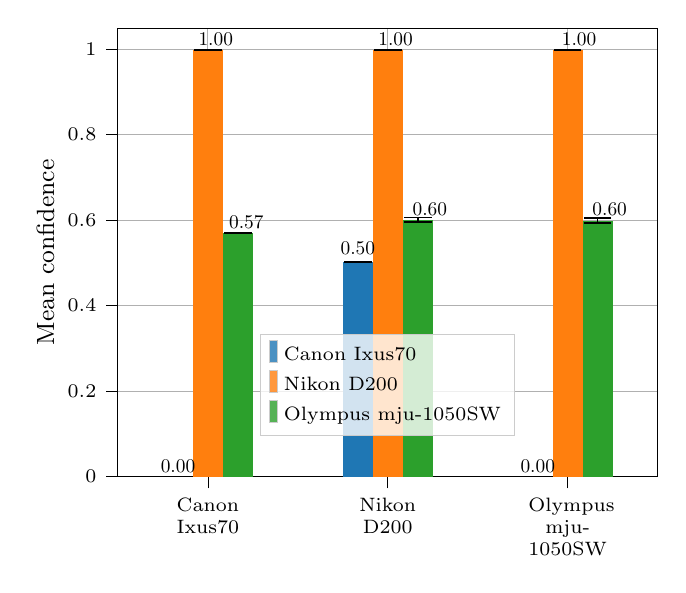
\begin{tikzpicture}

\definecolor{color0}{rgb}{0.12156862745098,0.466666666666667,0.705882352941177}
\definecolor{color1}{rgb}{1,0.498039215686275,0.0549019607843137}
\definecolor{color2}{rgb}{0.172549019607843,0.627450980392157,0.172549019607843}

\pgfplotsset{compat=1.11,
	/pgfplots/ybar legend/.style={
		/pgfplots/legend image code/.code={%
			\draw[##1,/tikz/.cd,yshift=-0.25em]
			(0cm,0cm) rectangle (3pt,0.8em);},
	}, every tick label/.append style={font=\scriptsize}
}

\begin{axis}[
legend cell align={left},
legend style={fill opacity=0.8, draw opacity=1, text opacity=1, at={(0.5,0.09)}, anchor=south, draw=white!80!black},
tick align=outside,
tick pos=left,
grid=major,
x grid style={white!69.0196078431373!black},
xmin=-0.5, xmax=2.5,
xtick style={color=black},
xtick={0,1,2},
xticklabel style={text width=1cm, align=center},
xticklabels={Canon Ixus70,Nikon D200,Olympus mju-1050SW},
y grid style={white!69.0196078431373!black},
ymin=0, ymax=1.04931477289574,
ytick style={color=black},
y label style={at={(axis description cs:-0.1,.5)},anchor=south},
ylabel={\small Mean confidence}
]
\draw[draw=none,fill=color0] (axis cs:-0.25,0) rectangle (axis cs:-0.0833333333333333,0);
\addlegendimage{ybar,ybar legend,draw=none,fill=color0};
\addlegendentry{\scriptsize Canon Ixus70}

\draw[draw=none,fill=color0] (axis cs:0.75,0) rectangle (axis cs:0.916666666666667,0.501532256603241);
\draw[draw=none,fill=color0] (axis cs:1.75,0) rectangle (axis cs:1.91666666666667,0);
\draw[draw=none,fill=color1] (axis cs:-0.0833333333333333,0) rectangle (axis cs:0.0833333333333333,0.999205410480499);
\addlegendimage{ybar,ybar legend,draw=none,fill=color1};
\addlegendentry{\scriptsize Nikon D200}

\draw[draw=none,fill=color1] (axis cs:0.916666666666667,0) rectangle (axis cs:1.08333333333333,0.997942090034485);
\draw[draw=none,fill=color1] (axis cs:1.91666666666667,0) rectangle (axis cs:2.08333333333333,0.998534440994263);
\draw[draw=none,fill=color2] (axis cs:0.0833333333333333,0) rectangle (axis cs:0.25,0.570436358451843);
\addlegendimage{ybar,ybar legend,draw=none,fill=color2};
\addlegendentry{\scriptsize Olympus mju-1050SW}

\draw[draw=none,fill=color2] (axis cs:1.08333333333333,0) rectangle (axis cs:1.25,0.601129174232483);
\draw[draw=none,fill=color2] (axis cs:2.08333333333333,0) rectangle (axis cs:2.25,0.599153518676758);
\path [draw=black, semithick]
(axis cs:-0.166666666666667,0)
--(axis cs:-0.166666666666667,0);

\path [draw=black, semithick]
(axis cs:0.833333333333333,0.501532256603241)
--(axis cs:0.833333333333333,0.501532256603241);

\path [draw=black, semithick]
(axis cs:1.83333333333333,0)
--(axis cs:1.83333333333333,0);

\path [draw=black, semithick]
(axis cs:0,0.99906341820315)
--(axis cs:0,0.999347402757849);

\path [draw=black, semithick]
(axis cs:1,0.997483955608914)
--(axis cs:1,0.998400224460056);

\path [draw=black, semithick]
(axis cs:2,0.998253126657801)
--(axis cs:2,0.998815755330725);

\path [draw=black, semithick]
(axis cs:0.166666666666667,0.570436358451843)
--(axis cs:0.166666666666667,0.570436358451843);

\path [draw=black, semithick]
(axis cs:1.16666666666667,0.59607423748821)
--(axis cs:1.16666666666667,0.606184110976756);

\path [draw=black, semithick]
(axis cs:2.16666666666667,0.5936379712075)
--(axis cs:2.16666666666667,0.604669066146016);

\addplot [semithick, black, mark=-, mark size=5, mark options={solid}, only marks]
table {%
-0.166666666666667 0
0.833333333333333 0.501532256603241
1.83333333333333 0
};

\addplot [semithick, black, mark=-, mark size=5, mark options={solid}, only marks]
table {%
-0.166666666666667 0
0.833333333333333 0.501532256603241
1.83333333333333 0
};

\addplot [semithick, black, mark=-, mark size=5, mark options={solid}, only marks]
table {%
0 0.99906341820315
1 0.997483955608914
2 0.998253126657801
};

\addplot [semithick, black, mark=-, mark size=5, mark options={solid}, only marks]
table {%
0 0.999347402757849
1 0.998400224460056
2 0.998815755330725
};

\addplot [semithick, black, mark=-, mark size=5, mark options={solid}, only marks]
table {%
0.166666666666667 0.570436358451843
1.16666666666667 0.59607423748821
2.16666666666667 0.5936379712075
};

\addplot [semithick, black, mark=-, mark size=5, mark options={solid}, only marks]
table {%
0.166666666666667 0.570436358451843
1.16666666666667 0.606184110976756
2.16666666666667 0.604669066146016
};

\draw (axis cs:-0.3,0.01) node[
  scale=0.7,
  anchor=base west,
  text=black,
  rotate=0.0
]{0.00};
\draw (axis cs:0.7,0.52) node[
  scale=0.7,
  anchor=base west,
  text=black,
  rotate=0.0
]{0.50};
\draw (axis cs:1.7,0.01) node[
  scale=0.7,
  anchor=base west,
  text=black,
  rotate=0.0
]{0.00};
\draw (axis cs:-0.09,1.01) node[
  scale=0.7,
  anchor=base west,
  text=black,
  rotate=0.0
]{1.00};
\draw (axis cs:0.91,1.01) node[
  scale=0.7,
  anchor=base west,
  text=black,
  rotate=0.0
]{1.00};
\draw (axis cs:1.93,1.01) node[
  scale=0.7,
  anchor=base west,
  text=black,
  rotate=0.0
]{1.00};
\draw (axis cs:0.08,0.58) node[
  scale=0.7,
  anchor=base west,
  text=black,
  rotate=0.0
]{0.57};
\draw (axis cs:1.1,0.61) node[
  scale=0.7,
  anchor=base west,
  text=black,
  rotate=0.0
]{0.60};
\draw (axis cs:2.1,0.61) node[
  scale=0.7,
  anchor=base west,
  text=black,
  rotate=0.0
]{0.60};
\end{axis}

\end{tikzpicture}
}
	}
	\caption{Prediction confidence of images blurred by Gaussian filter with kernel's size of $ 5 \times 5 $ and standard deviation $ \sigma = 1.1 $.}
	\label{fig:blur confidence}
\end{figure}

%%%%%%%%%%%%%%%%%%%%%%%%%%%%%%%%%%%%%%%%%%%%%%%%%%%%%%%%%%%%%%%%%%%%%%%%%%%%%%
\paragraph{Summary}
\label{section:blur summary}
%%%%%%%%%%%%%%%%%%%%%%%%%%%%%%%%%%%%%%%%%%%%%%%%%%%%%%%%%%%%%%%%%%%%%%%%%%%%%%

In this section, the results show that the classifier is severely affected by the Gaussian blur operation, which causes it to tend to recognize blurred images as images from Nikon D200. One possible explanation for this could be that the traces left by Nikon D200 has lower frequency compared to the other two images since the Gaussian blur process is a low pass filtering operation.

%%%%%%%%%%%%%%%%%%%%%%%%%%%%%%%%%%%%%%%%%%%%%%%%%%%%%%%%%%%%%%%%%%%%%%%%%%%%%%
\subsection{Different devices for same model}
\label{section:instance}
%%%%%%%%%%%%%%%%%%%%%%%%%%%%%%%%%%%%%%%%%%%%%%%%%%%%%%%%%%%%%%%%%%%%%%%%%%%%%%

In order to study the robustness of our CNN-based camera model classifier to the device-dependent characteristics, we separate the images of our training set according to models and devices. Each model has more than one device, more specifically, three devices for Canon Ixus70, two devices for Nikon D200 and five devices for Olympus mju-1050SW. 

%%%%%%%%%%%%%%%%%%%%%%%%%%%%%%%%%%%%%%%%%%%%%%%%%%%%%%%%%%%%%%%%%%%%%%%%%%%%%%
\subsubsection*{Data Collection \& Training}
\label{section:instance data collection}
%%%%%%%%%%%%%%%%%%%%%%%%%%%%%%%%%%%%%%%%%%%%%%%%%%%%%%%%%%%%%%%%%%%%%%%%%%%%%%

We select the images from one device of each model. These three devices from Canon Ixus70, Nikon D200 and Olympus mju-1050SW has 187, 372 and 204 full sized images respectively. Then we divide these images into $ 256 \times 256 $ pixels patches and train our CNN with them in the same manner described in Section~\ref{section:Data collection & Training}. In total, there are 19,075 patches in this dataset, of which 15,260 images are used for training and 3,815 images for evaluating the performance of our CNN.

The other images, namely 380 full sized images from Canon Ixus70, 380 from Nikon D200 and 836 from Olympus mju-1050SW, are used as the testing data for this experiment. Again, separate them in $ 256 \times 256 $ pixels patches. In total, the number of images for testing robustness to device-dependent characteristics is 35,075.

\begin{figure}
	\centering
	\resizebox{!}{!}{
		{% This file was created by tikzplotlib v0.9.1.
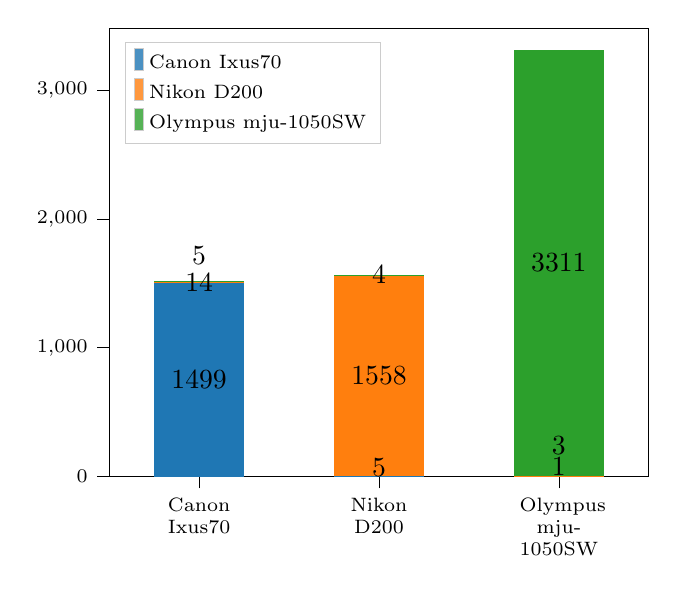
\begin{tikzpicture}

\definecolor{color0}{rgb}{0.12156862745098,0.466666666666667,0.705882352941177}
\definecolor{color1}{rgb}{1,0.498039215686275,0.0549019607843137}
\definecolor{color2}{rgb}{0.172549019607843,0.627450980392157,0.172549019607843}

\pgfplotsset{compat=1.11,
	/pgfplots/ybar legend/.style={
		/pgfplots/legend image code/.code={%
			\draw[##1,/tikz/.cd,yshift=-0.25em]
			(0cm,0cm) rectangle (3pt,0.8em);},
	}, every tick label/.append style={font=\scriptsize}
}

\begin{axis}[
legend cell align={left},
legend style={fill opacity=0.8, draw opacity=1, text opacity=1, at={(0.03,0.97)}, anchor=north west, draw=white!80!black},
tick align=outside,
tick pos=left,
x grid style={white!69.0196078431373!black},
xmin=-0.5, xmax=2.5,
xtick style={color=black},
xtick={0,1,2},
xticklabel style={text width=1cm, align=center},
xticklabels={Canon Ixus70,Nikon D200,Olympus mju-1050SW},
y grid style={white!69.0196078431373!black},
ymin=0, ymax=3480.75,
ytick style={color=black}
]
\draw[draw=none,fill=color0] (axis cs:-0.25,0) rectangle (axis cs:0.25,1499);
\addlegendimage{ybar,ybar legend,draw=none,fill=color0};
\addlegendentry{\scriptsize Canon Ixus70}

\draw[draw=none,fill=color0] (axis cs:0.75,0) rectangle (axis cs:1.25,5);
\draw[draw=none,fill=color0] (axis cs:1.75,0) rectangle (axis cs:2.25,1);
\draw[draw=none,fill=color1] (axis cs:-0.25,1499) rectangle (axis cs:0.25,1513);
\addlegendimage{ybar,ybar legend,draw=none,fill=color1};
\addlegendentry{\scriptsize Nikon D200}

\draw[draw=none,fill=color1] (axis cs:0.75,5) rectangle (axis cs:1.25,1563);
\draw[draw=none,fill=color1] (axis cs:1.75,1) rectangle (axis cs:2.25,4);
\draw[draw=none,fill=color2] (axis cs:-0.25,1513) rectangle (axis cs:0.25,1518);
\addlegendimage{ybar,ybar legend,draw=none,fill=color2};
\addlegendentry{\scriptsize Olympus mju-1050SW}

\draw[draw=none,fill=color2] (axis cs:0.75,1563) rectangle (axis cs:1.25,1567);
\draw[draw=none,fill=color2] (axis cs:1.75,4) rectangle (axis cs:2.25,3315);
\draw (axis cs:0,749.5) node[
  scale=1,
  text=black,
  rotate=0.0
]{1499};
\draw (axis cs:1,70) node[
  scale=1,
  text=black,
  rotate=0.0
]{5};
\draw (axis cs:2,80) node[
  scale=1,
  text=black,
  rotate=0.0
]{1};
\draw (axis cs:0,1506) node[
  scale=1,
  text=black,
  rotate=0.0
]{14};
\draw (axis cs:1,784) node[
  scale=1,
  text=black,
  rotate=0.0
]{1558};
\draw (axis cs:2,240) node[
  scale=1,
  text=black,
  rotate=0.0
]{3};
\draw (axis cs:0,1715) node[
  scale=1,
  text=black,
  rotate=0.0
]{5};
\draw (axis cs:1,1565) node[
  scale=1,
  text=black,
  rotate=0.0
]{4};
\draw (axis cs:2,1659.5) node[
  scale=1,
  text=black,
  rotate=0.0
]{3311};
\end{axis}

\end{tikzpicture}
}
	}
	\caption{Prediction of images from different devices of same model. The numbers from top to bottom indicate the number of images classified as Olympus mju-1050SW, Nikon D200 and Canon Ixus70 respectively.}
	\label{fig:ins result}
\end{figure}

\begin{figure}
	\centering
	\resizebox{!}{!}{
		{% This file was created by tikzplotlib v0.9.1.
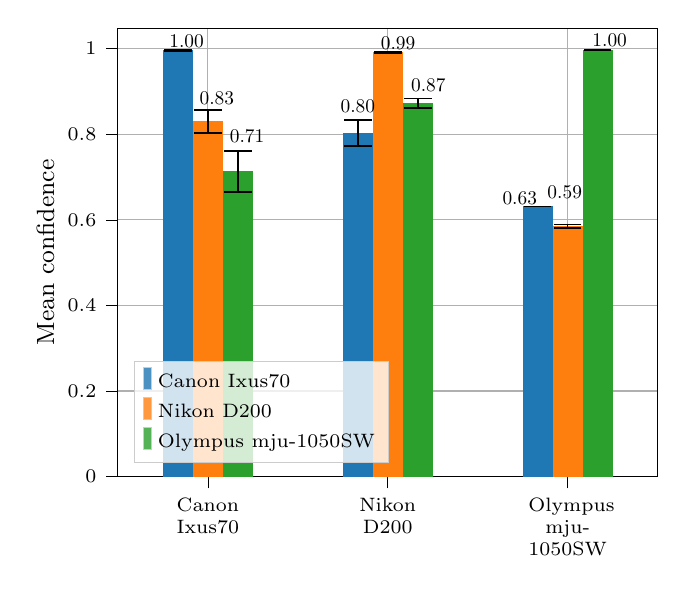
\begin{tikzpicture}

\definecolor{color0}{rgb}{0.12156862745098,0.466666666666667,0.705882352941177}
\definecolor{color1}{rgb}{1,0.498039215686275,0.0549019607843137}
\definecolor{color2}{rgb}{0.172549019607843,0.627450980392157,0.172549019607843}

\pgfplotsset{compat=1.11,
	/pgfplots/ybar legend/.style={
		/pgfplots/legend image code/.code={%
			\draw[##1,/tikz/.cd,yshift=-0.25em]
			(0cm,0cm) rectangle (3pt,0.8em);},
	}, every tick label/.append style={font=\scriptsize}
}

\begin{axis}[
legend cell align={left},
legend style={fill opacity=0.8, draw opacity=1, text opacity=1, at={(0.03,0.03)}, anchor=south west, draw=white!80!black},
tick align=outside,
tick pos=left,
grid=major,
x grid style={white!69.0196078431373!black},
xmin=-0.5, xmax=2.5,
xtick style={color=black},
xtick={0,1,2},
xticklabel style={text width=1cm, align=center},
xticklabels={Canon Ixus70,Nikon D200,Olympus mju-1050SW},
y grid style={white!69.0196078431373!black},
ymin=0, ymax=1.04773845525342,
ytick style={color=black},
y label style={at={(axis description cs:-0.1,.5)},anchor=south},
ylabel={\small Mean confidence}
]
\draw[draw=none,fill=color0] (axis cs:-0.25,0) rectangle (axis cs:-0.0833333333333333,0.99585235118866);
\addlegendimage{ybar,ybar legend,draw=none,fill=color0};
\addlegendentry{\scriptsize Canon Ixus70}

\draw[draw=none,fill=color0] (axis cs:0.75,0) rectangle (axis cs:0.916666666666667,0.803355395793915);
\draw[draw=none,fill=color0] (axis cs:1.75,0) rectangle (axis cs:1.91666666666667,0.631426155567169);
\draw[draw=none,fill=color1] (axis cs:-0.0833333333333333,0) rectangle (axis cs:0.0833333333333333,0.830226242542267);
\addlegendimage{ybar,ybar legend,draw=none,fill=color1};
\addlegendentry{\scriptsize Nikon D200}

\draw[draw=none,fill=color1] (axis cs:0.916666666666667,0) rectangle (axis cs:1.08333333333333,0.991193056106567);
\draw[draw=none,fill=color1] (axis cs:1.91666666666667,0) rectangle (axis cs:2.08333333333333,0.58521842956543);
\draw[draw=none,fill=color2] (axis cs:0.0833333333333333,0) rectangle (axis cs:0.25,0.712932467460632);
\addlegendimage{ybar,ybar legend,draw=none,fill=color2};
\addlegendentry{\scriptsize Olympus mju-1050SW}

\draw[draw=none,fill=color2] (axis cs:1.08333333333333,0) rectangle (axis cs:1.25,0.872416436672211);
\draw[draw=none,fill=color2] (axis cs:2.08333333333333,0) rectangle (axis cs:2.25,0.997382640838623);
\path [draw=black, semithick]
(axis cs:-0.166666666666667,0.994838729617186)
--(axis cs:-0.166666666666667,0.996865972760133);

\path [draw=black, semithick]
(axis cs:0.833333333333333,0.772691080346704)
--(axis cs:0.833333333333333,0.834019711241126);

\path [draw=black, semithick]
(axis cs:1.83333333333333,0.631426155567169)
--(axis cs:1.83333333333333,0.631426155567169);

\path [draw=black, semithick]
(axis cs:0,0.803120279684663)
--(axis cs:0,0.857332205399871);

\path [draw=black, semithick]
(axis cs:1,0.989438349730335)
--(axis cs:1,0.9929477624828);

\path [draw=black, semithick]
(axis cs:2,0.581346617080271)
--(axis cs:2,0.589090242050588);

\path [draw=black, semithick]
(axis cs:0.166666666666667,0.664979506283998)
--(axis cs:0.166666666666667,0.760885428637266);

\path [draw=black, semithick]
(axis cs:1.16666666666667,0.86130363214761)
--(axis cs:1.16666666666667,0.883529241196811);

\path [draw=black, semithick]
(axis cs:2.16666666666667,0.996919133816846)
--(axis cs:2.16666666666667,0.9978461478604);

\addplot [semithick, black, mark=-, mark size=5, mark options={solid}, only marks]
table {%
-0.166666666666667 0.994838729617186
0.833333333333333 0.772691080346704
1.83333333333333 0.631426155567169
};
 
\addplot [semithick, black, mark=-, mark size=5, mark options={solid}, only marks]
table {%
-0.166666666666667 0.996865972760133
0.833333333333333 0.834019711241126
1.83333333333333 0.631426155567169
};
 
\addplot [semithick, black, mark=-, mark size=5, mark options={solid}, only marks]
table {%
0 0.803120279684663
1 0.989438349730335
2 0.581346617080271
};
 
\addplot [semithick, black, mark=-, mark size=5, mark options={solid}, only marks]
table {%
0 0.857332205399871
1 0.9929477624828
2 0.589090242050588
};
 
\addplot [semithick, black, mark=-, mark size=5, mark options={solid}, only marks]
table {%
0.166666666666667 0.664979506283998
1.16666666666667 0.86130363214761
2.16666666666667 0.996919133816846
};
 
\addplot [semithick, black, mark=-, mark size=5, mark options={solid}, only marks]
table {%
0.166666666666667 0.760885428637266
1.16666666666667 0.883529241196811
2.16666666666667 0.9978461478604
};
 
\draw (axis cs:-0.252,1.00381916999817) node[
  scale=0.7,
  anchor=base west,
  text=black,
  rotate=0.0
]{1.00};
\draw (axis cs:0.7,0.85) node[
  scale=0.7,
  anchor=base west,
  text=black,
  rotate=0.0
]{0.80};
\draw (axis cs:1.6,0.636477564811707) node[
  scale=0.7,
  anchor=base west,
  text=black,
  rotate=0.0
]{0.63};
\draw (axis cs:-0.084,0.87) node[
  scale=0.7,
  anchor=base west,
  text=black,
  rotate=0.0
]{0.83};
\draw (axis cs:0.924,0.99912260055542) node[
  scale=0.7,
  anchor=base west,
  text=black,
  rotate=0.0
]{0.99};
\draw (axis cs:1.85,0.65) node[
  scale=0.7,
  anchor=base west,
  text=black,
  rotate=0.0
]{0.59};
\draw (axis cs:0.084,0.78) node[
  scale=0.7,
  anchor=base west,
  text=black,
  rotate=0.0
]{0.71};
\draw (axis cs:1.092,0.9) node[
  scale=0.7,
  anchor=base west,
  text=black,
  rotate=0.0
]{0.87};
\draw (axis cs:2.1,1.00536170196533) node[
  scale=0.7,
  anchor=base west,
  text=black,
  rotate=0.0
]{1.00};
\end{axis}

\end{tikzpicture}
}
	}
	\caption{Prediction confidence of images from different devices of same model.}
	\label{fig:ins confidence}
\end{figure}

%%%%%%%%%%%%%%%%%%%%%%%%%%%%%%%%%%%%%%%%%%%%%%%%%%%%%%%%%%%%%%%%%%%%%%%%%%%%%%
\subsubsection*{Result}
\label{section:instance result}
%%%%%%%%%%%%%%%%%%%%%%%%%%%%%%%%%%%%%%%%%%%%%%%%%%%%%%%%%%%%%%%%%%%%%%%%%%%%%%

The performance of our CNN in this experiment turns out to be really similar compared to Table~\ref{tab:train} and Figure~\ref{fig:test confidence}. Using the images from different devices as input, the results are depicted in Figure~\ref{fig:ins result} and Figure~\ref{fig:ins confidence}. As we can see, the accuracy for this experiment is at least 98.75\%.

In terms of confidence of prediction, the mean confidence for the ground truth labels are about 1, similar to Figure~\ref{fig:test confidence}. Compared to Canon Ixus70 and Nikon D200, the Olympus mju-1050SW is slightly better as for the prediction confidences for wrong classes are around 0.6, while the other two models have around 0.8 confidences.

%%%%%%%%%%%%%%%%%%%%%%%%%%%%%%%%%%%%%%%%%%%%%%%%%%%%%%%%%%%%%%%%%%%%%%%%%%%%%%
\subsubsection*{Summary}
\label{section:instance summary}
%%%%%%%%%%%%%%%%%%%%%%%%%%%%%%%%%%%%%%%%%%%%%%%%%%%%%%%%%%%%%%%%%%%%%%%%%%%%%%

We have demonstrated that the classification accuracy and the prediction confidence didn't change much for different devices. We can say that our CNN-based camera model classifier is robust to the device-dependent characteristics.

%%%%%%%%%%%%%%%%%%%%%%%%%%%%%%%%%%%%%%%%%%%%%%%%%%%%%%%%%%%%%%%%%%%%%%%%%%%%%%
\section{Conclusion}
\label{section:conclusion}
%%%%%%%%%%%%%%%%%%%%%%%%%%%%%%%%%%%%%%%%%%%%%%%%%%%%%%%%%%%%%%%%%%%%%%%%%%%%%%

In this report, we presented how a CNN-based camera model classifier behaves in the presence of three different types of data, namely, unseen data, post-processed data, and data from different devices.

By suppressing image’s content and extracting high frequency traces from camera using constrained convolutional layer, the CNN architecture has at least 99.69\% accuracy as well as mean confidence of 1 for the correct label in the baseline experiment. It makes our results independent to image's scenes and objects. However, we showed that our CNN is not robust to the out-of-distribution data in most of the experiments. It tends to classify images from unseen model to the model with the same manufacturer as the input and makes decisions with high confidence regardless of the ground truth. In the post-processing experiment, we have demonstrated that our CNN is robust to JPEG compression artifacts only for Nikon D200, but it doesn't generalize to the other two models. Furthermore, the CNN tends to classify noisy images as they are from Canon Ixus70 and blurred images as they are from Nikon D200 with high confidence. The only exception is the device-dependent characteristics experiment, our classifier shows similar accuracy and mean confidence compared to the baseline experiment, which means it is robust to device-dependent characteristics.

These are preliminary experiments. There are many aspects to be further investigated in the future work, such as the method of evaluating the prediction confidence, effects to the robustness of more different image manipulation techniques and the effects of camera parameters while shooting photos.	

%%%%%%%%%%%%%%%%%%%%%%%%%%%%%%%%%%%%%%%%%%%%%%%%%%%%%%%%%%%%%%%%%%%%%%%%%%%%%%%%%%%%%%%%%%%%%%%%%%
%\bibliographystyle{abbrv}
\bibliographystyle{plainnat}
\small
\bibliography{references}
%%%%%%%%%%%%%%%%%%%%%%%%%%%%%%%%%%%%%%%%%%%%%%%%%%%%%%%%%%%%%%%%%%%%%%%%%%%%%%%%%%%%%%%%%%%%%%%%%%

\end{document}
